\chapter{The Phase 1 New Small Wheel Upgrade Project}
\label{chap:nsw}

%“Unless commitment is made, there are only promises and hopes; but no plans.” -- Peter F. Drucker
%Management is about human beings. Its task is to make people capable of joint performance, to make their strengths effective and their weaknesses irrelevant. -- Drucker
%Every enterprise requires commitment to common goals and shared values. Without such commitment there is no enterprise; there is only a mob. The enterprise must have simple, clear, and unifying objectives. The mission of the organization has to be clear enough and big enough to provide common vision. The goals that embody it have to be clear, public, and constantly reaffirmed. Management’s first job is to think through, set, and exemplify those objectives, values, and goals. -- Drucker
%plan, organize, integrate, motivate, and measure. -- drucker

%Two hundred people, of course, can do a great deal more work than one man. But it does not follow that they produce and contribute more. -- drucker

\epigraph{\textit{Every enterprise requires commitment to common goals and shared values. Without such commitment there is no enterprise; there is only a mob.}}{--Peter F. Drucker, \textit{Essential Drucker}}
\epigraph{\textit{So it goes...}}{--Kurt Vonnegut, \textit{Slaughterhouse Five}}

During its first two periods of operation --- Runs 1 and 2 --- the LHC operated
at or exceeded its design goals.
In Run 2, in 2018, ATLAS observed a peak of more than 60 $pp$ interactions per bunch crossing with nominal running conditions for physics data taking
and instantaneous luminosities exceeding $2\times 10^{34}$ cm$^{-2}$\,s$^{-1}$.
These instantaneous luminosity levels were those originally envisaged as the end goal for data taking \textit{after} LS2,
during which the Phase 1 Upgrades are planned to take place both for the LHC and the large experiments, as shown in Figure~\ref{fig:lhc_schedule}.
During LS2, which at the time of writing is currently taking place, the LHC plans to upgrade its injection chain to allow for delivering ever
more increased peak instantaneous luminosities to the experiments.
During LS3, the LHC will have its entire magnet system overhauled and will be upgraded to become the
High Luminosity LHC (HL-LHC) allowing for subsequent LHC runs to deliver increased bunch densities 
to the experiments, thereby achieving peak luminosities far exceeding those observed thus far~\cite{HLLHCPDR}.

In the following sections, the large-scale Phase 1 Upgrade to the ATLAS detector's forward muon system
will be introduced.
The upgrade is a replacement of the current MDT- and CSC-based Small Wheel section of the ATLAS MS endcap, located at $z \approx 7$\,m (Figure~\ref{fig:muon_plan_view_eta}),
and is the largest such upgrade targetting HL-LHC data-taking conditions to take place so far amongst the LHC experiments.
The detector upgrade is referred to as the New Small Wheel (NSW) and is planned for completion by
the end of LS2~\cite{NSWTDR}.
The NSW is planned to last for the remainder of the ATLAS detector's lifetime, and is designed with the
HL-LHC data-taking conditions in mind.
In Section~\ref{sec:nsw_motivation} the reasons necessitating an upgrade to the forward muon system
of ATLAS will be presented, with emphasis on how the current system will not be able to maintain high
levels of performance in the Run 3 and HL-LHC era.
Section~\ref{sec:nsw_layout} will then proceed to describe the detector technologies that make up
the NSW, and how they will meet the foreseen challenges of Run 3 and beyond, as well as their layout
within the ATLAS detector.
Sections~\ref{sec:nsw_elx}-\ref{sec:nsw_verso} will introduces the aspects of the NSW that the
current author predominantly worked on; namely, the development of the software interface to the NSW front-end readout
electronics and detectors necessary for both validation and integration of the NSW readout infrastructure.

%%%%%%%%%%%%%%%%%%%%%%%%%%%%%%%%%%%%%%%%%%%%%%%%%%%%%%%%%%%%%%%%%%%%%%%
% NSW MOTIVATION
%%%%%%%%%%%%%%%%%%%%%%%%%%%%%%%%%%%%%%%%%%%%%%%%%%%%%%%%%%%%%%%%%%%%%%%
\section{The Need for an Upgraded Forward Muon System}
\label{sec:nsw_motivation}

The luminosity increases planned to take place during Run 3 and the HL-LHC
era means that ATLAS will be subjected to exceedingly high particle rates.
As mentioned previously, the peak number of interactions per bunch-crossing observed during
Run 2 operations was $\langle \mu \rangle \approx 60$.
Given the recent experience of the LHC delivering above expectation,
the increases in collision intensity planned for Run 3 imply a peak number approaching
$\langle \mu \rangle \approx 80-100$. 
That of the HL-LHC, nearing luminosities of $10^{35}$\,cm$^{-2}$s$^{-1}$, implies peaks approaching $\langle \mu \rangle \approx 200$ or more, depending
on the beam configuration.
While most of the detectors in the ATLAS muon system were designed with large enough safety margins
to handle the foreseen rates, the inner-most forward station --- the Small Wheel --- will
exceed its design capabilities.
The current Small Wheel covers $1.0 < \lvert \eta \rvert < 2.7$ (Figure~\ref{fig:muon_plan_view_eta}).
At $\lvert \eta \rvert = \pm 2.7$, rates of $\approx 20$\,kHz/cm$^2$ are expected, far higher
than what the currently-installed MDT and CSC detectors and readout electronics can handle.
Moreover, the end-cap region of ATLAS covers nearly 63\% of the ATLAS muon system rapidity.
High detector performance in this region, therefore, is of the utmost importance in order to
achieve the long-term physics goals of ATLAS and the upgraded LHC.

The end-cap Level-1 muon trigger logic is based on track segments formed by hits in the TGC chambers
in the middle muon station at $z\approx 13$\,m, the first `Big Wheel' (Figure~\ref{fig:muon_plan_view_eta}).
The \pT~of muon candidates, used to define the thresholds at which the triggers accept an event, is
determined by the angle of the track segment with respect to the direction pointing back to the IP.
In the forward region of ATLAS there is a significant background rate composed of low energy particles ---
mainly protons, neutrons, and photons --- generated as a result of material interactions between
the Small and Big Wheels.
Figure~\ref{fig:cavern_bkg} illustrates the levels of material interactions within the ATLAS
cavern that lead to this so-called `cavern background'.
These low energy particles can produce `fake' triggers by traversing the end-cap chambers
at angles similar to that of real high-\pT~muons originating from the IP.
This situation is illustrated in Figure~\ref{fig:l1mu_rates}, wherein it is seen that
a significant fraction of the reconstructed muons in the forward muon system cannot be matched
to a trigger candidate from the ID.
These `fake' triggers amount to roughly 90\% of the total muon triggers in ATLAS.
With the foreseen luminosity upgrades of the LHC, the number of such triggers in the end-cap region
will exceed the \textit{total} ATLAS Level-1 trigger rate budget of 100\,kHz (only 20\,kHz are budgeted
for Level-1 muon triggers).

\begin{figure}[!htb]
    \begin{center}
        %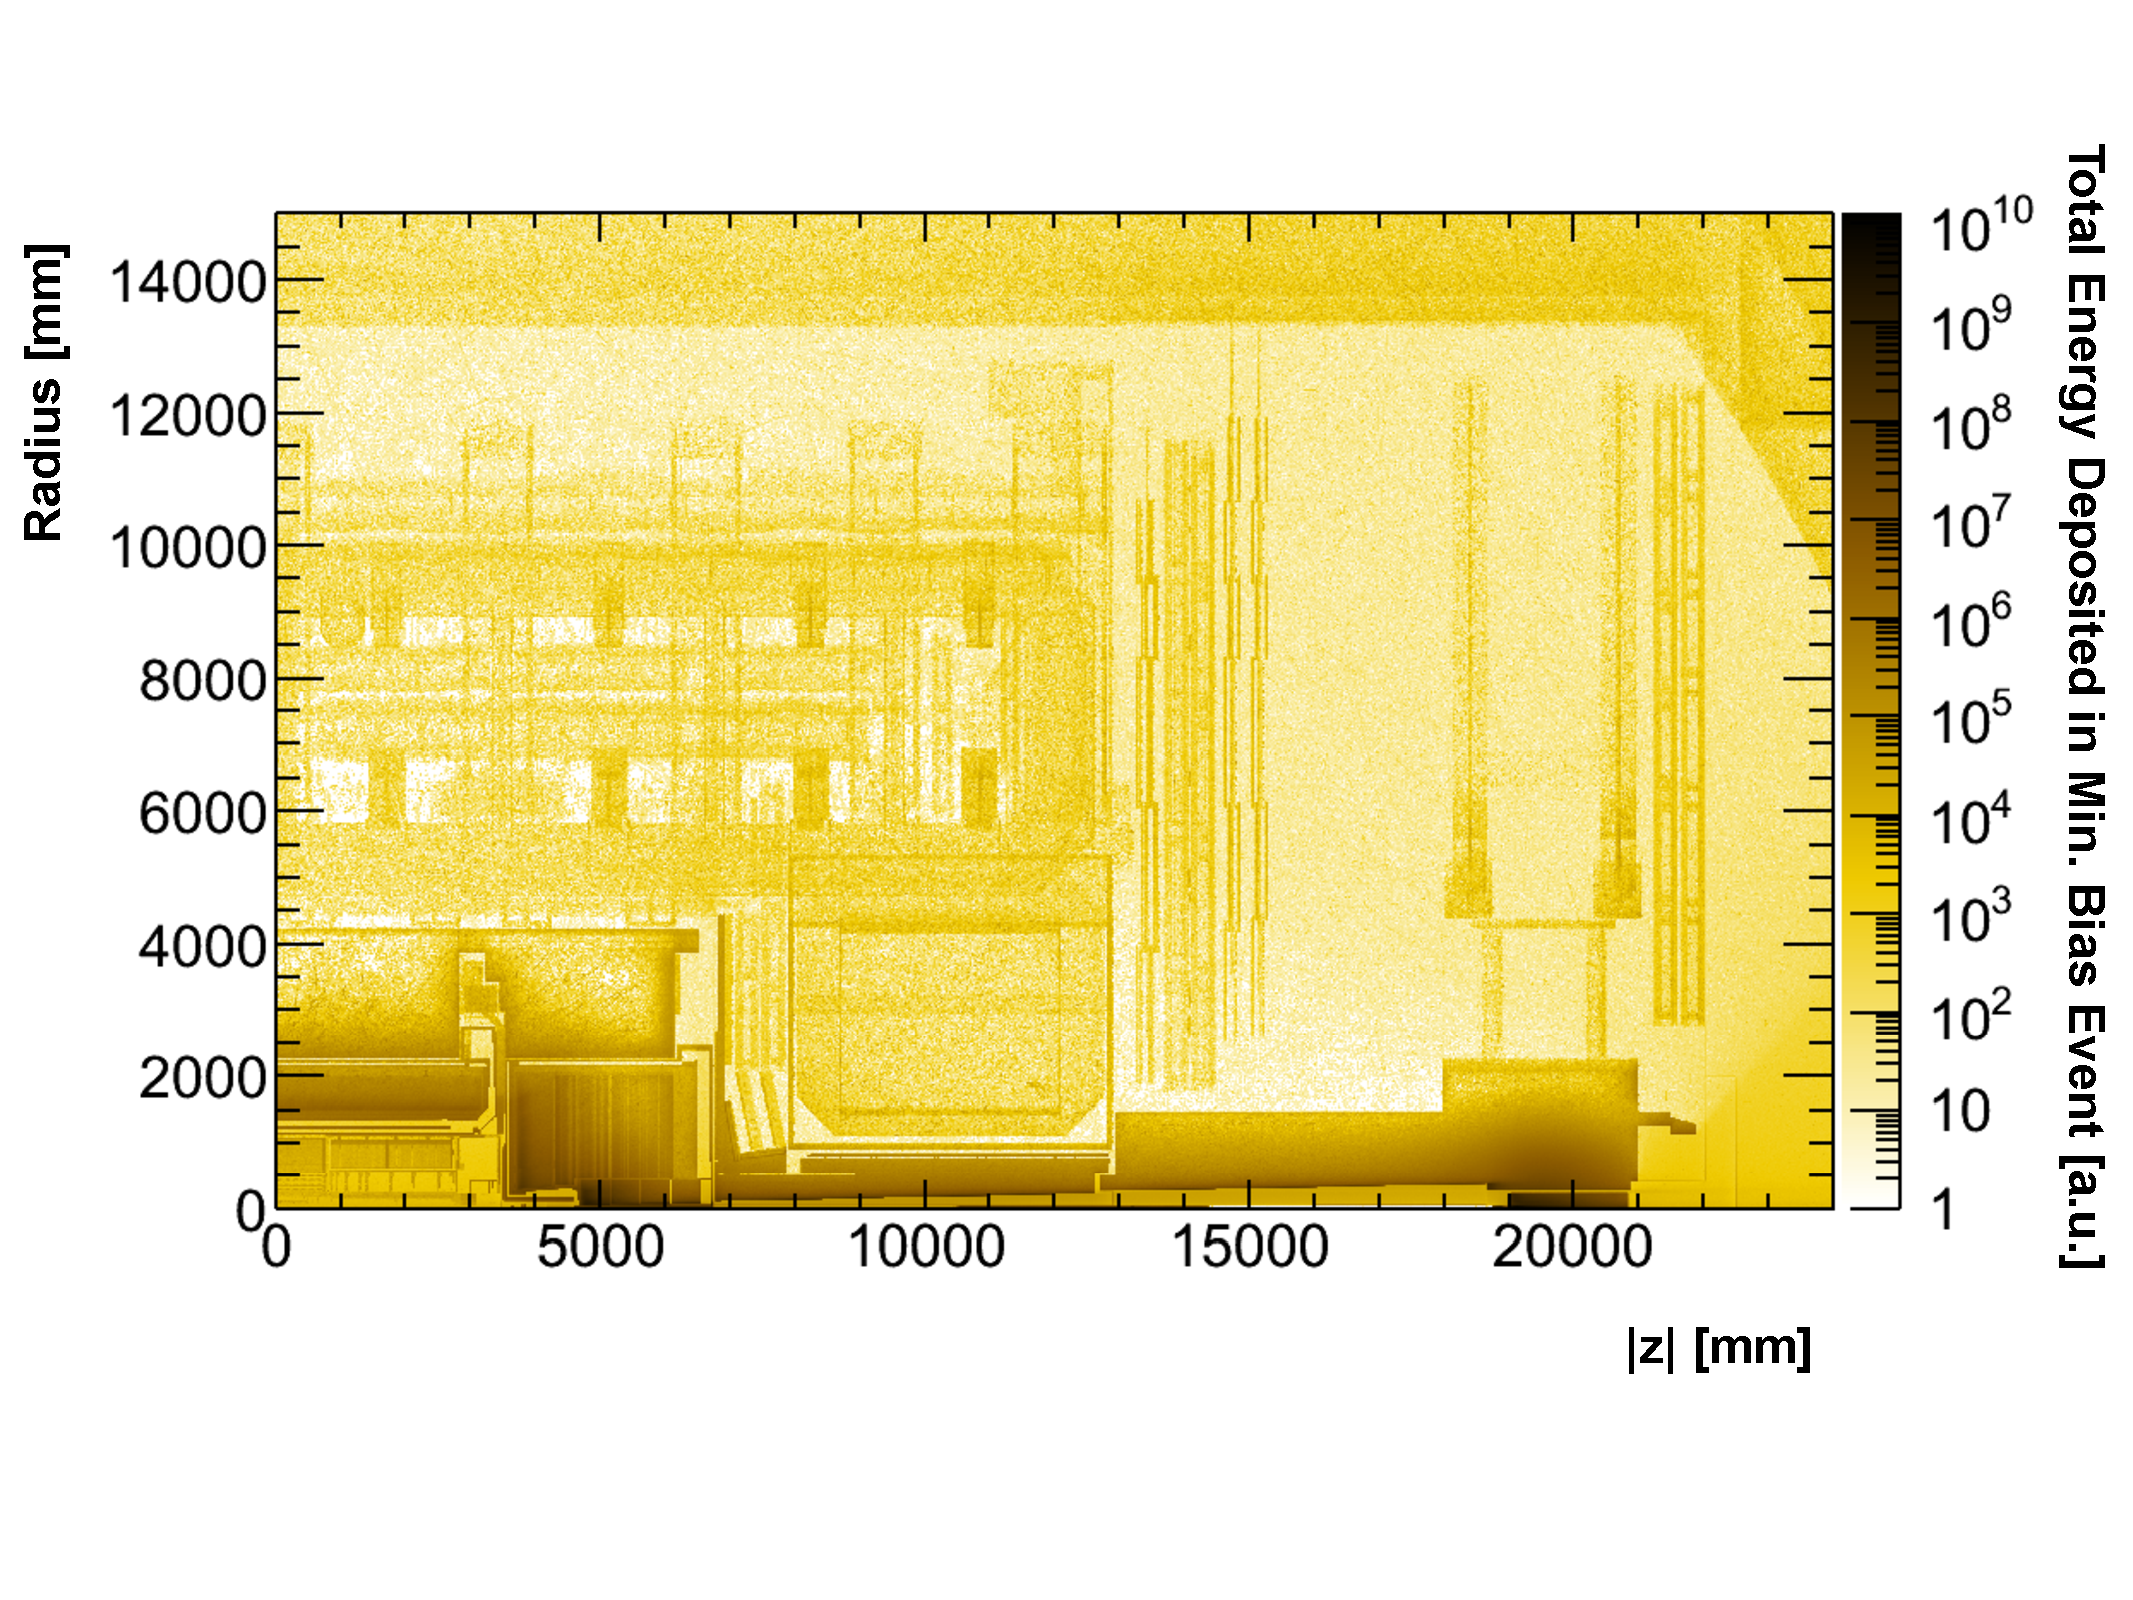
\includegraphics[width=0.8\textwidth]{figures/nsw/atlas_cavern_bkgPDF}
        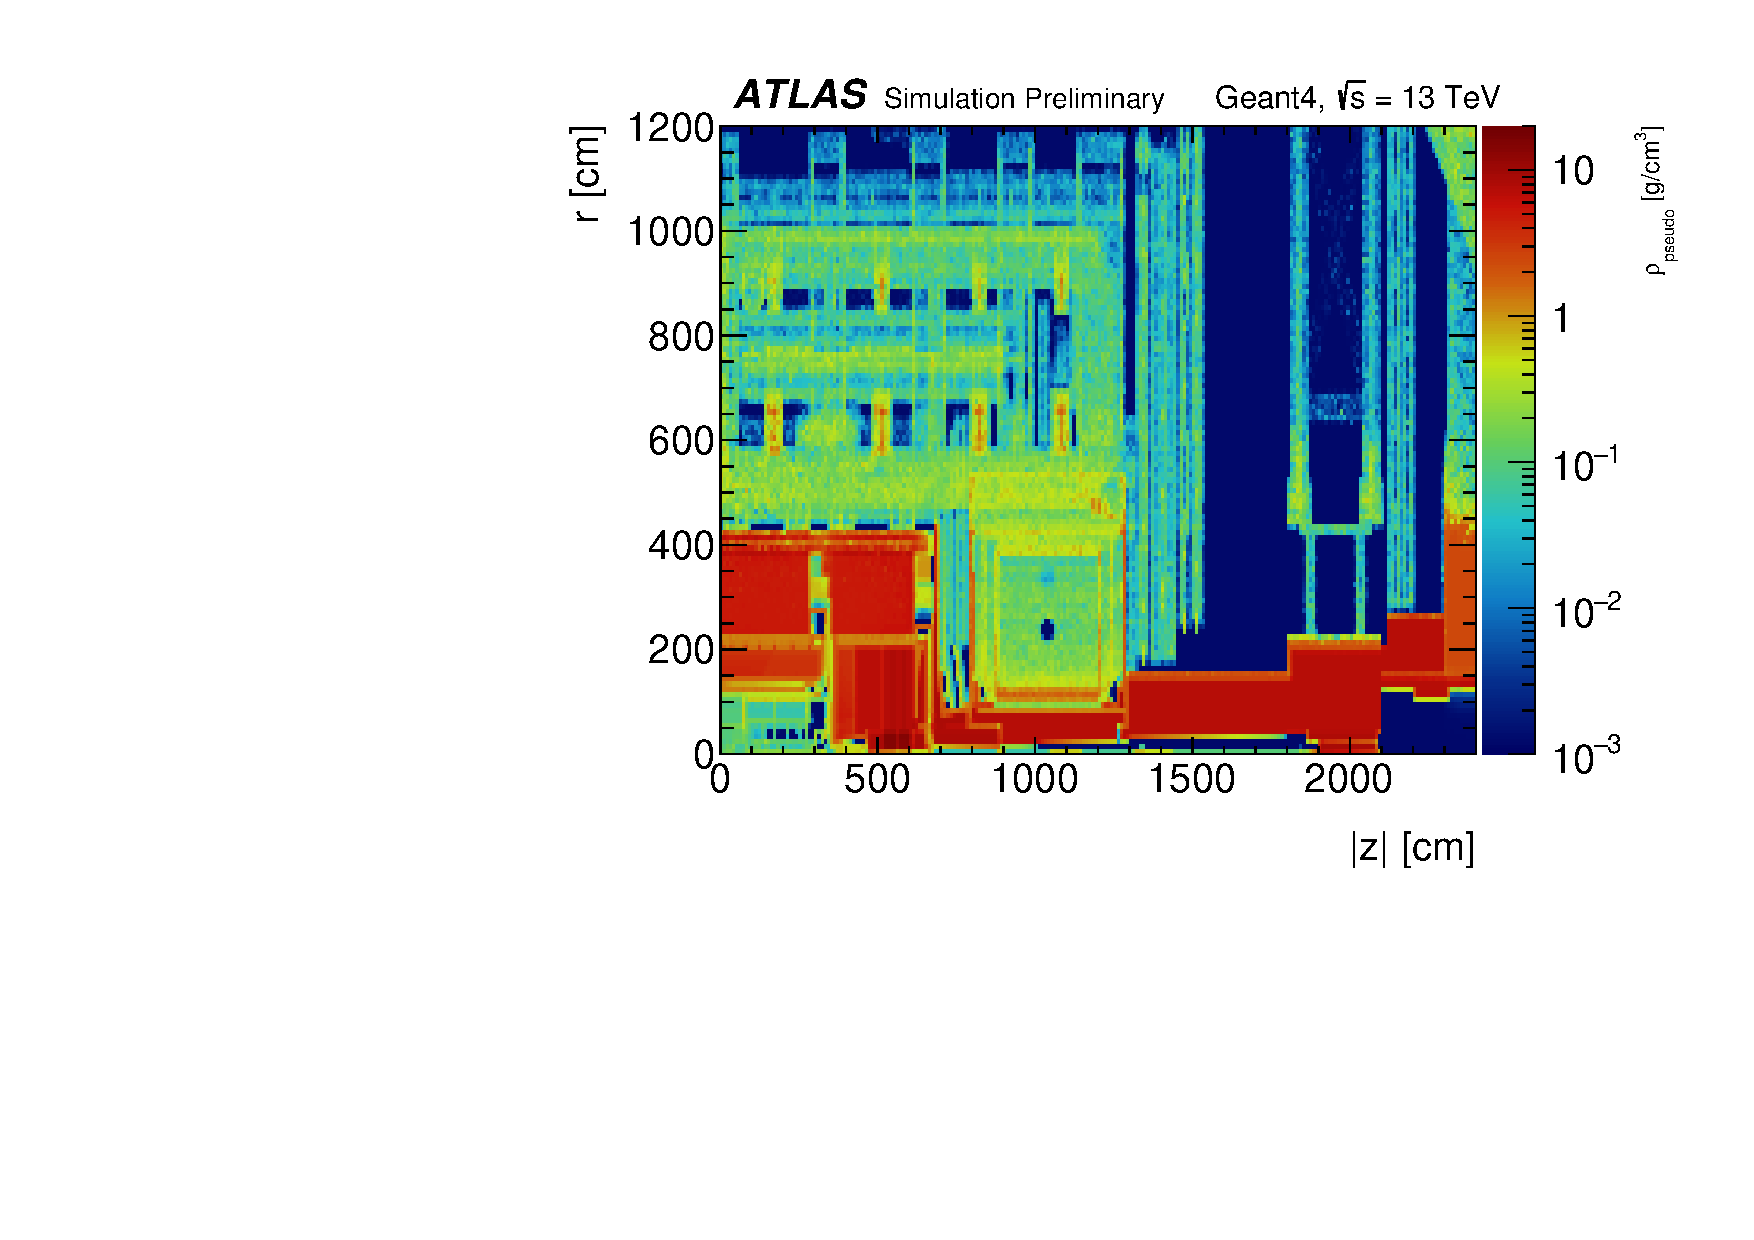
\includegraphics[width=0.8\textwidth]{figures/nsw/atlas_cavern_material_density_sim}
        \caption{
            Simulation of the average material density in materials within a quadrant of the ATLAS cavern.
            %during a minimum bias collision event at $13\,\TeV$.
            %The normalisation of the $z$-axis is arbitrary.
            The forward-calorimeter cryostat, beam-pipe, and shielding ($z\approx 6.8$\,m)
            in front of the Small Wheel experience high energy deposition.
            The largest rates observed by the muon system are those experienced
            by the CSC detectors in the current Small Wheel, which can be seen in the above
            to lie directly behind and above regions of high material interaction.
            Figure taken from Ref.~\cite{ATL-PHYS-PUB-2016-017}.
        }
        \label{fig:cavern_bkg}
    \end{center}
\end{figure}

The NSW will take part in the Level-1 muon trigger by providing
tracking information to aid the TGC-based Level-1 muon trigger logic currently in use for providing
Level-1 muon trigger candidates in the forward region.
The inclusion of such trigger information from the NSW will help to discriminate against
`fake' triggers due to background particles, as illustrated in Figure~\ref{fig:l1mu_rates},
and will also improve the overall muon \pT~measurement in the forward muon trigger which
will enable the Level-1 muon triggers to maintain low \pT-thresholds.
If there were no NSW upgrade, in order to cope with the high rate of Level-1 muon triggers,
the \pT~thresholds of the single-muon triggers would have to be increased from a minimum of $\approx20\,\GeV$
to thresholds well above 40\,\GeV in order to drop the total rate of muon triggers (inclusive of those
in the barrel and end-cap) below the 20\,kHz budget.
Alternatively, the forward muon trigger system could be removed altogether.
In this latter case, all muon triggers would be seeded by Level-1 muon candidates in the barrel only.
Both of these scenarios lead to drastic reduction in physics performance.
Major Higgs-physics goals of ATLAS, for example, would take large hits if either of these
two non-NSW scenarios were enacted.
Increasing the Level-1 muon trigger \pT-thresholds results in a loss in efficiency of more than
30\% for the $Wh,h\rightarrow bb$ process --- a key channel necessary for the observation and study
of the Higgs couplings to $b$-quarks.
A drop in efficiency on the order of 50\% is expected for the same process if the trigger thresholds
are kept low but the forward muon trigger system is removed.
This is illustrated in Figure~\ref{fig:nsw_wh_loss}, both for the $Wh,h\rightarrow bb$ scenario
discussed but also for the $h\rightarrow WW^*$ production channel, an important source of Higgs bosons
in ATLAS.


\begin{figure}[!htb]
    \begin{center}
        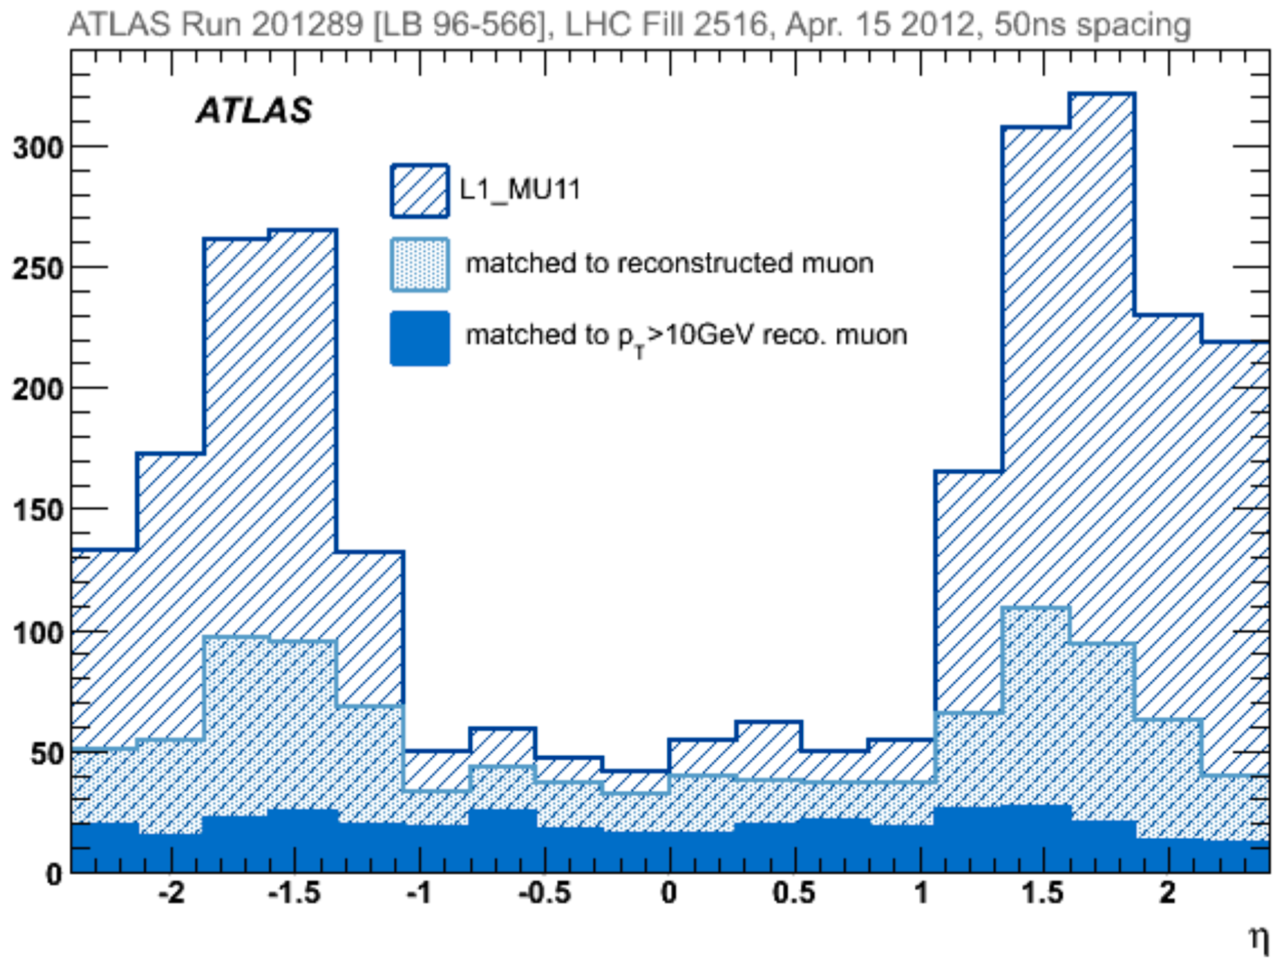
\includegraphics[width=0.47\textwidth]{figures/nsw/nsw_l1mu_rates}
        \raisebox{0.4cm}{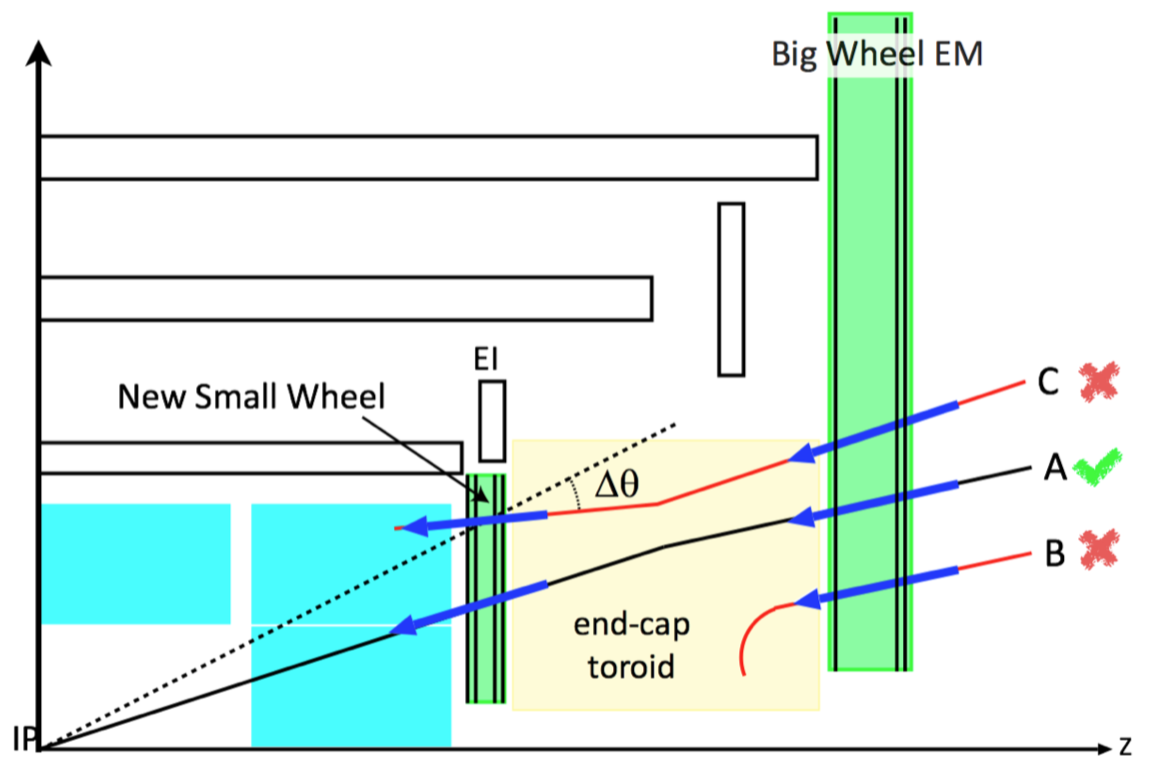
\includegraphics[width=0.5\textwidth]{figures/nsw/nsw_track_principle}}
        \caption{
            Figures taken from Ref.~\cite{NSWTDR}.
            \textbf{\textit{Left}}: Level-1 muon trigger rates as a function of $\eta$. L1\_MU11 refers to the
                rate of the Level-1 accept rate. After requiring that the muon trigger candidates
                responsible for the Level-1 muon trigger firing are matched to a real muon, the
                rate drops significantly, illustrating the rate of `fake' muon triggers in the
                forward muon system.
            \textbf{\textit{Right}}: Illustration of the principle of operation of the NSW trigger system.
                The aim of the NSW trigger is to provide accurate pointing information (via the illustrated $\Delta \theta$ computation) within
                the inner-most muon system to aid the trigger logic of the Big Wheel and thereby reduce the acceptance of `fake' triggers that
                do not have coincident pointing track segments in both wheels.
                With the NSW trigger logic, only the muon trigger candidate labelled `A' will result
                in a Level-1 muon trigger being fired.
                The track candidate `C' (`B') fails to fire a trigger due to non-IP-pointing (missing) track-segments in the NSW,
                characteristic of cavern background particles.
        }
        \label{fig:l1mu_rates}
    \end{center}
\end{figure}

\begin{figure}[!htb]
    \begin{center}
        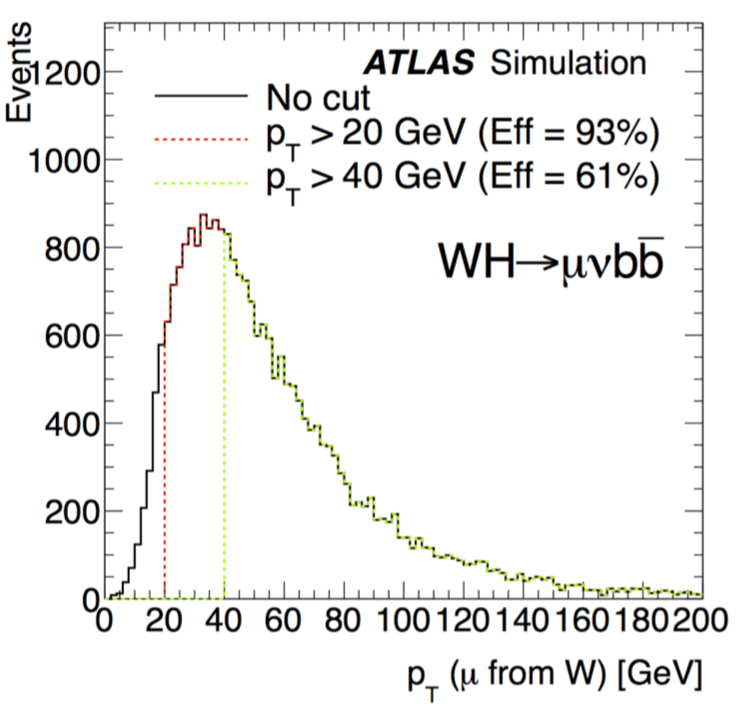
\includegraphics[width=0.4\textwidth]{figures/nsw/nsw_ptmu_wh}
        \raisebox{1.85cm}{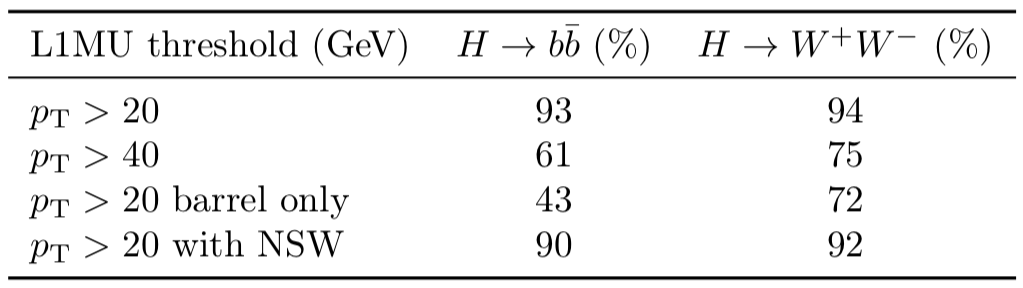
\includegraphics[width=0.55\textwidth]{figures/nsw/nsw_eff_wh_hbb}}
        \caption{
            Figures taken from studies contained in Ref.~\cite{NSWTDR}.
            \textit{\textbf{Left}}: Truth-level \pT~distribution of the trigger-muon in the $Wh$ analysis, showing
                the trigger thresholds and corresponding truth-level selection efficiency of those thresholds.
            \textit{\textbf{Right}}: Selection efficiencies for several trigger-threshold scenarios with and without the NSW
                for the $Wh,h\rightarrow b \bar{b}$ and $h \rightarrow WW^*$ processes.
        }
        \label{fig:nsw_wh_loss}
    \end{center}
\end{figure}

In addition to the trigger performance of the current forward muon system being insufficient
for the foreseen data-taking challenges, the tracking performance of both the MDT and CSC detectors of the current Small Wheel
will also degrade with the increased luminosities.
For example, the MDT detectors are characterised by long signal drift-times that are hundreds of nanoseconds long.
With both these long characteristic drift times and the increased particle rates predicted to occur with the LHC upgrades,
the occupancies that will be experienced by the MDT chambers in the current Small Wheel
will result in significant degradation of their tracking capabilities.
At the high rates expected in the future runs of the (HL-)LHC, the tracking efficiencies
of the MDT chambers will approach 50\% or worse (lower), as illustrated in Figure~\ref{fig:nsw_mdt_track_reco}.
This leads to significant reductions in the capabilities of the inner-most muon stations
in the forward region to provide a third high-resolution muon measurement necessary for the sagitta measurement used for reconstructing
muon momenta.

\begin{figure}[!htb]
    \begin{center}
        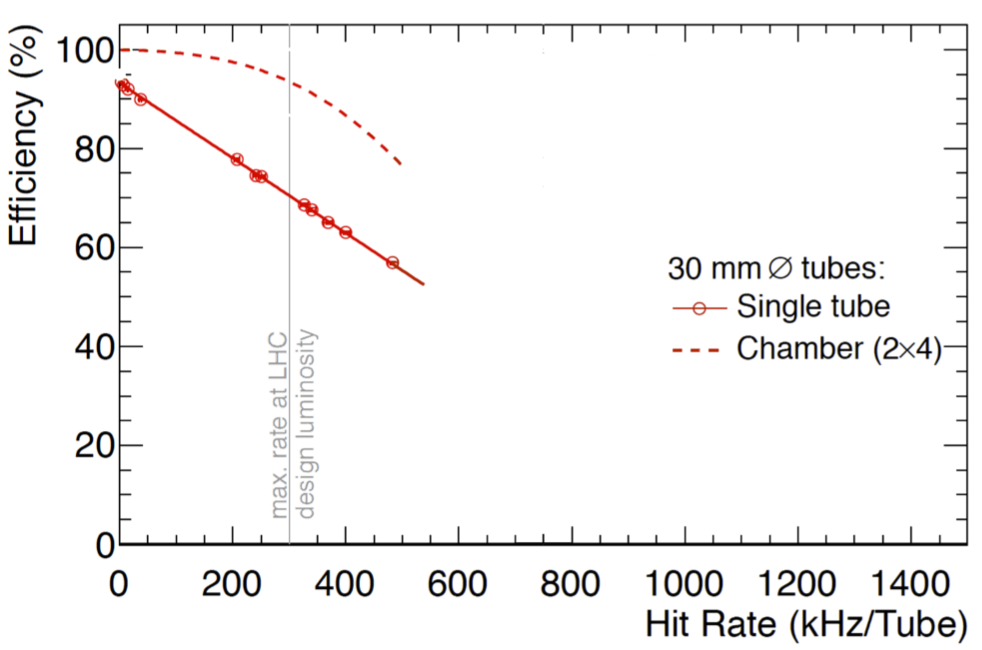
\includegraphics[width=0.7\textwidth]{figures/nsw/nsw_mdt_track_reco_eff}
        \caption{
            Measurements of MDT tube hit (solid line) and track-segment efficiency (dashed-line)
            as a function of tube hit rate.
            The vertical line indicating the maximum LHC rate corresponds to an instantaneous
            luminosity of $1\times10^{34}$cm$^{-2}$s$^{-1}$.
            Figure taken from Ref.~\cite{NSWTDR}.
        }
        \label{fig:nsw_mdt_track_reco}
    \end{center}
\end{figure}


%%%%%%%%%%%%%%%%%%%%%%%%%%%%%%%%%%%%%%%%%%%%%%%%%%%%%%%%%%%%%%%%%%%%%%%
% NSW DETECTOR
%%%%%%%%%%%%%%%%%%%%%%%%%%%%%%%%%%%%%%%%%%%%%%%%%%%%%%%%%%%%%%%%%%%%%%%
\section{The New Small Wheel Detector}
\label{sec:nsw_detector}

%The inability of the current Small Wheel to cope with the foreseen challenges
%of Run 3 and the HL-LHC have been briefly discussed in the
%previous sections.
In this section, a description of the NSW will be presented.
The layout of the NSW will be described in Section~\ref{sec:nsw_geo}
and then a description of the \micromegas (MM)~\cite{Giomataris:1995fq} and Small-strip Thin Gap Chamber (sTGC)
detector technologies that will compose the NSW
will be given in Sections~\ref{sec:nsw_mm} and \ref{sec:nsw_stgc}, respectively.
The MM are throught of as providing primarily high presicion muon tracking
while the sTGC are thought of as primarily providing trigger primitives for the forward Level-1 muon trigger system.
As will be seen, though, both the MM and sTGC technologies will provide both high-quality tracking and trigger primitives.
%The MM detectors are primarily precision tracking detectors and the sTGC
%will serve as trigger detectors, though each provide both tracking and trigger primitives.
The NSW must last for the remainder of the ATLAS detector's lifetime, throughout
both Run 3 and the entirety of the HL-LHC era.
In the following sections, the design decisions of the NSW --- related to both its layout 
and detector choices --- will be presented in light of their ability to address
the particular challenges described in the previous section.

%%%%%%%%%%%%%%%%%%%%%%%%%%%%%%%%%%%%%%%%%%%%%%%%%%%%%%%%%%%%%%%
% NSW GEO
%%%%%%%%%%%%%%%%%%%%%%%%%%%%%%%%%%%%%%%%%%%%%%%%%%%%%%%%%%%%%%%
\subsection{Geometry and Layout}
\label{sec:nsw_geo}

The NSW consists of 16 detector planes, separated into two `multilayers'.
Each multilayer will be composed of four detector planes of each of the two
detector technologies that make up the NSW: the Small-strip Thin Gap Chamber (sTGC)
and MicroMegas\footnote{The name `MicroMegas` is a loose acryonym for `MICROMEsh GAseous Structure'.} (MM)
detectors.
The sTGC are based on multiwire chamber technology and the MM are a type of
micropattern gaseous detector (MPGD)~\cite{MPGD}.
The detectors are arranged into sectors in azimuth, following a similar layout
as the current Small Wheel with alternating large and small sectors, as illustrated in Figure~\ref{fig:nsw_geo}.
The organisation of the detector technologies in each sector is illustrated in Figure~\ref{fig:nsw_sector_layout},
showing the sTGC--MM--MM--sTGC layout of the detector quadruplets, with a $50$\,mm spacer
frame separating the two halves.
Each sector of the NSW will have a length nearing 5\,m, giving the NSW a diameter of
nearly 10\,m.

The current Small Wheel muon system covers the range $1.0 < \lvert \eta \rvert < 2.7$, shown
in Figure~\ref{fig:muon_plan_view_eta}.
The NSW will not cover the entirey of this range, however, and will only cover the
range $1.3 < \lvert \eta \rvert < 2.7$ while the already-existing MDT chambers in the Small Wheel at $1.0 < \lvert \eta  \rvert < 1.3$
will remain in operation after the NSW installation.
The NSW will additionally extend the Level-1 muon trigger system acceptance to include
the region $2.4 < \lvert \eta \rvert < 2.7$, which is currently not the case.

The large number of detection planes provided by the NSW adds a large degree of redundancy
within each of the quadruplets of a given technology: if part of a layer, or even a complete layer,
is non-functioning the remaining layers within the quadruplet will compensate and a loss in performance
will be minimal.
There is additional redundancy provided by the fact that both MM and sTGC detector technologies
will be used for both tracking and trigger functionalities: if an entire or part of a quadruplet
becomes non-functioning, the tracking and/or trigger responsibilities of the lost detector
will be partially covered by the presence of the still-functioning quadruplet(s)/layer(s) of the other
detector technology covering the same or overlapping
$\eta$ range.
%There is additional redundancy provided by the fact that \textit{both} the MM and sTGC detectors
%will provide both tracking and trigger primitives: if an entire or part of a quadruplet becomes
%non-functioning, then the functionalities of the lost detector will be partially covered
%by that of the still-functioning quadruplet(s) in the same $\lvert \eta \rvert$ range.
%That is, although the MM and sTGC are described as being specialised for tracking and trigger functionalities,
%respectively, each technology provides quality inputs for both functions.
The degree of redundancy built into the NSW detector is such that the performance goals
of ATLAS with respect to the forward muon system can be met for the remainder of the experiment's
lifetime of 15 years or more.
With generally few opportunities for meaningful repair and maintenance access, this redundancy is
a necessity for these timescales.

\begin{figure}[!htb]
    \begin{center}
        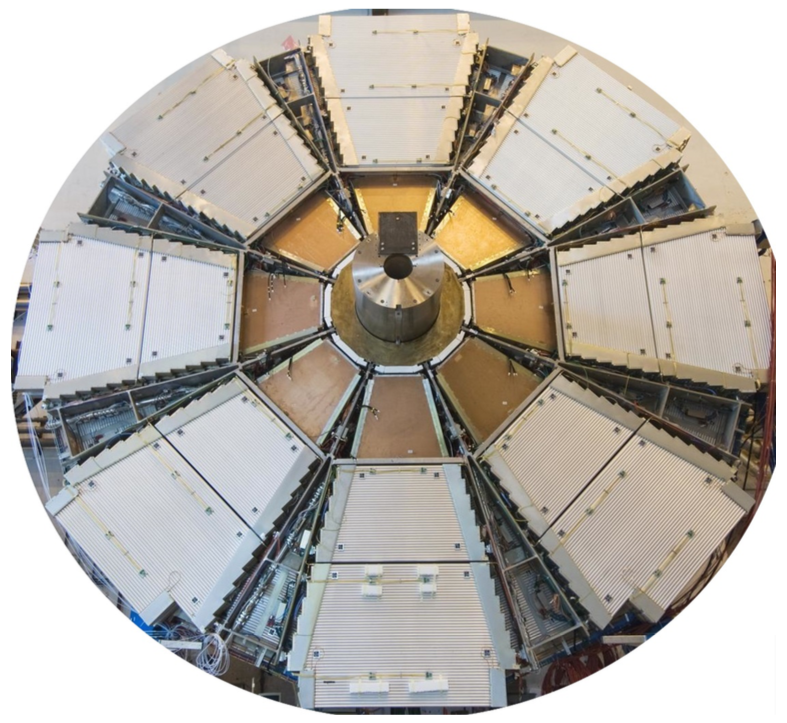
\includegraphics[width=0.48\textwidth]{figures/nsw/nsw_current_sw}
        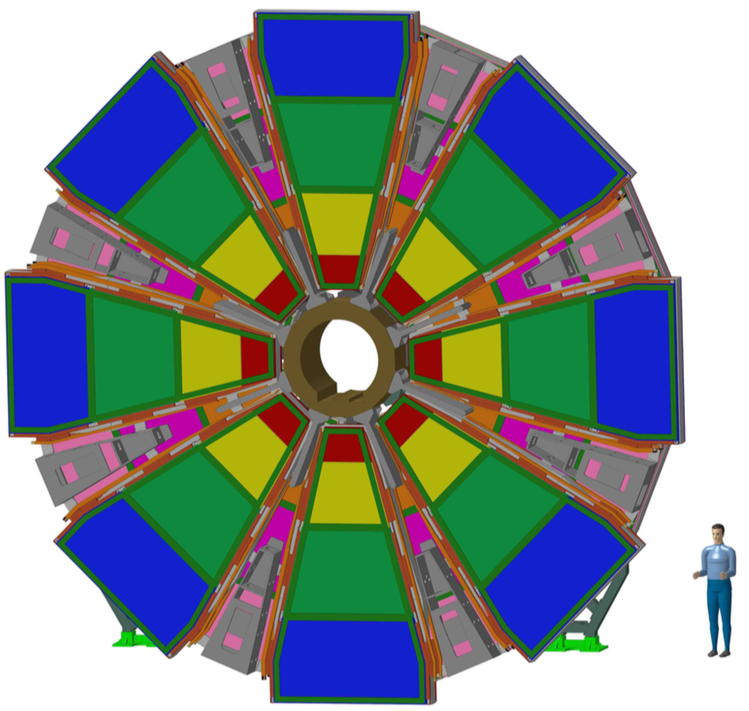
\includegraphics[width=0.48\textwidth]{figures/nsw/nsw_cartoon}
        \caption{
            \textbf{\textit{Left}}: Current Small Wheel detector (prior to installation in ATLAS), with CSC detectors (copper color) at low radii
                and MDT chambers (silver color) at higher radii.
            \textbf{\textit{Right}}: Geometry of the NSW, with a view of the large-sector side. The gaps in azimuth
                between the large sectors are instrumented with detectors on the side facing into the page.
        }
        \label{fig:nsw_geo}
    \end{center}
\end{figure}

\begin{figure}[!htb]
    \begin{center}
        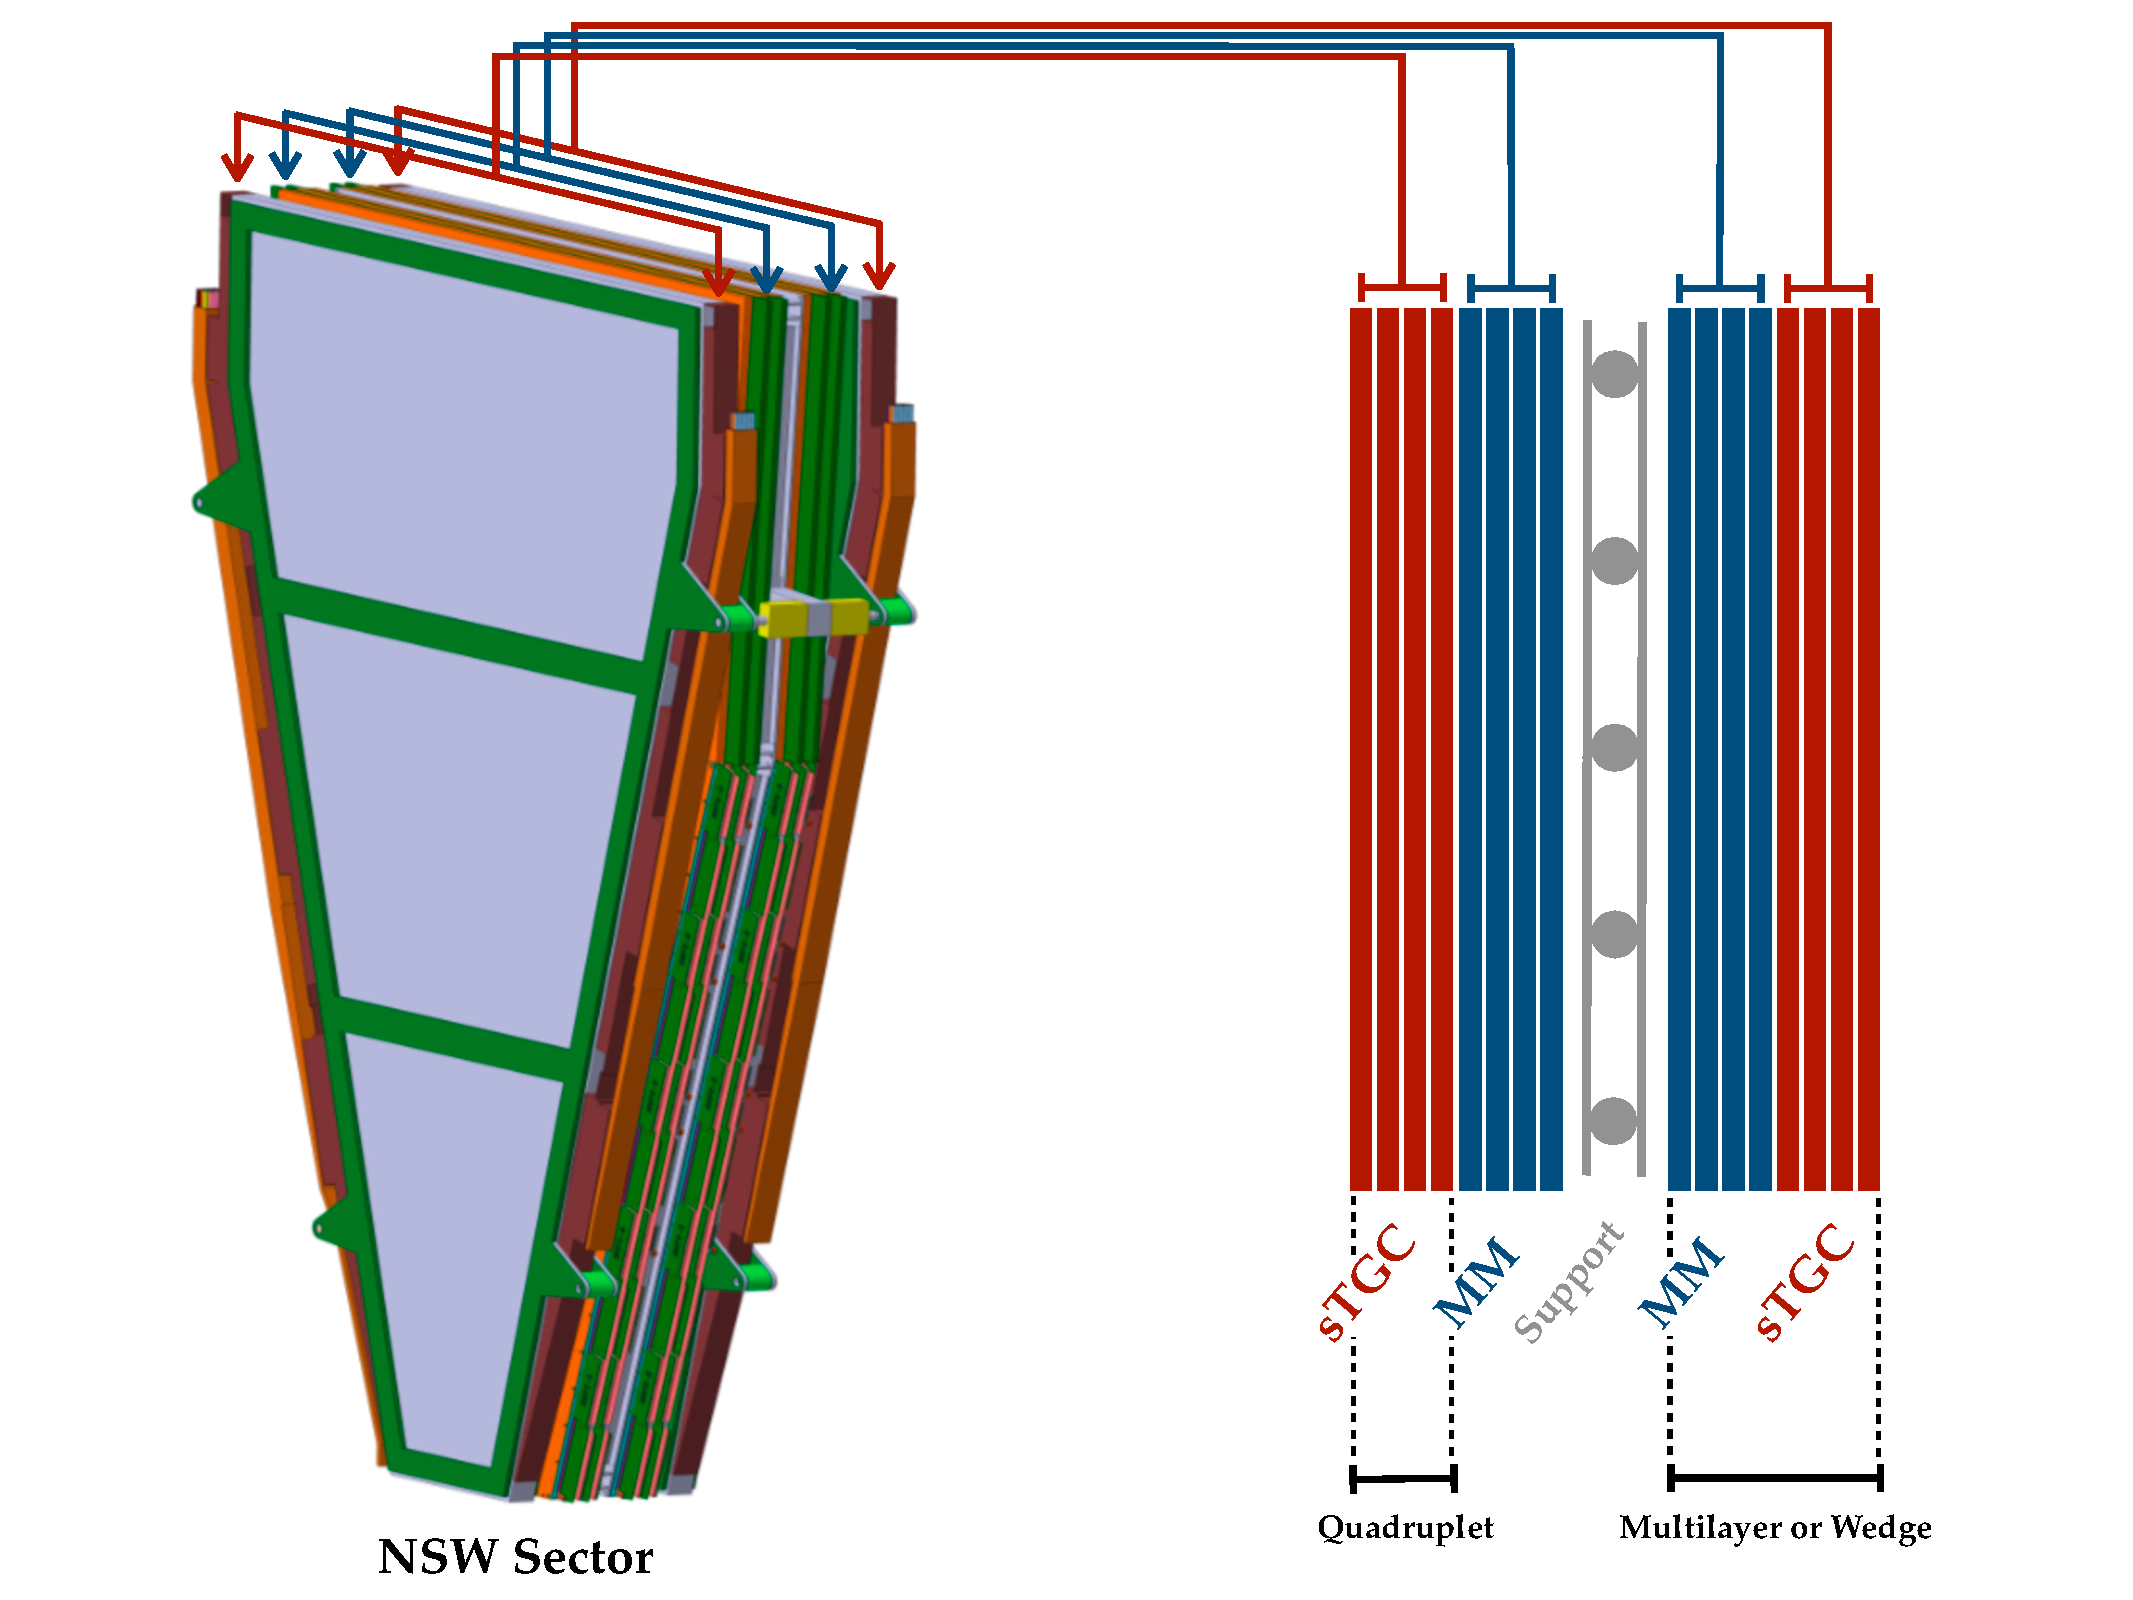
\includegraphics[width=0.8\textwidth]{figures/nsw/nsw_sector_layoutPDF}
        \caption{
            On the left is a mechanical drawing of an NSW sector, with the specific detector
            components illustrated on the right, composed of 16 detector planes: 8 MM layers
            sandwiched between 4 sTGC layers on either side.
            The base component of an NSW detector technology is a single detector plane,
            or layer, four of which are comprised in a single unit referred to as
            a `quadruplet'.
            A single side of the NSW, composed of an MM and sTGC quadruplet, is
            referred to as a `wedge' and a sector is referred to as a `double wedge'.
        }
        \label{fig:nsw_sector_layout}
    \end{center}
\end{figure}

%%%%%%%%%%%%%%%%%%%%%%%%%%%%%%%%%%%%%%%%%%%%%%%%%%%%%%%%%%%%%%%
% MICROMEGAS
%%%%%%%%%%%%%%%%%%%%%%%%%%%%%%%%%%%%%%%%%%%%%%%%%%%%%%%%%%%%%%%
\subsection{The Micromegas Detectors}
\label{sec:nsw_mm}

As mentioned above, the MM detectors are primarily designed with the high-precision tracking
requirements of the HL-LHC in mind, requring a per-layer spatial hit resolution better than $100\,\micron$.
The MM detectors are characterised by readout strips with very fine segmentation and good
time resolution.
Due to this fine time resolution, they will be able to complement the trigger scheme based
on the sTGC detector technology.

%The MM detectors are designed with the high-precision tracking requirements of the HL-LHC
%in mind, requiring a spatial precision better than $100\,\micron$.
%They are characterised by readout strips with very fine segmentation and good
%time resolution and can be exploited to complement the trigger scheme based on the sTGC, as
%described above.

MM detectors are characterised by two asymmetric regions.
The standard MM detector consists of a planar \textit{drift} electrode, a gas gap of
a few millimeters in thickness acting as a conversion and drift region, and a thin
metallic mesh at $\mathcal{O}(100)\,\micron$ above the readout electrodes.
The region between the mesh and readout electrodes is the amplification region wherein
gain factors on the order of $10^4$ are achievable.

The electric potentials within the drift and avalanche regions are maintained
at a few hundred V/cm and $\approx50$\,kV/cm, respectively.
Charged particles traversing the drift space ionise the gas and the electrons, liberated
in the ionisation process, drift towards the mesh at timescales on the order of tens of nanoseconds.
The electron avalanche takes place in the amplification region in about a nanosecond,
resulting in a fast current pulse on the readout electrode.

The MM detectors in the NSW are \textit{resistive-strip} MM detectors, characterised by an insulating
layer over the readout electrodes.
The insulating layer acts to protect the sensitive readout electrodes from sparking events that
reduce the detector performance over time and that are expected to happen frequently given
the very large gas amplification.
%Such sparking events can happen frequently given the very large gas amplifications and high electric potentials
%present in the amplification region.
Resistive strips on top of the insulating layer collect the avalanche electrons and induce
signals on copper readout strips embedded beneath the insulating layer.
The geometry (strip pitch and width) of the copper readout strips need not necessarily be the
same as that of the resistive strips.
Resistrive-strip MM detectors are able to sustain higher amplification and particle rates, a necessary
characteristic for targetting the high-luminosities foreseen at the HL-LHC.
The design and principle of operation of the resistive-strip MM technology is shown in Figure~\ref{fig:nsw_mm_principle},
in which incident MIPs traversing perpendicular and at an angle relative to the detector plane
are illustrated.

Each layer of an MM detector in the NSW is composed of $1024 \times 8$ parallel readout strips, giving
a highly granular spatial readout allowing for high resolution position measurements to be made.
Although all readout strips of a given MM layer are parallel, the MM quadruplets will be capable
of two-dimensional readout and will provide both $r$ and $\phi$ coordinate information
of traversing particles.
The two dimensional readout is achieved through the use of a small-angle stereo readout, in which
MM layers are tilted by fixed relative angles of $\pm 1.5$\,degrees.
This means of a two-dimensional readout is unlike that achieved by the CSC detectors in the current
Small Wheel, in which the readout plane consists of perpendicular wires and strips providing
the two dimensional readout information.
This perpendicular readout is susceptible to high rates of so-called \textit{ghost hits},
illustrated in the left side of Figure~\ref{fig:mm_stereo}, and leads to high levels of track-building ambiguities.
In the high particle rates expected at the HL-LHC, the multiplicies of these ghost hits would
lead to an unacceptable degradation in tracking performance.
The combination of the small-angle stereo readout and high strip-multiplicities on each MM layer will
enable the MM detectors to sustain these high particle rates.
In the right side of Figure~\ref{fig:mm_stereo}, the layout of the MM layers in the NSW as regards
their readout strip orientation (i.e. tilted or not) is illustrated.

Typical definitions of hit locations within strip-based detectors are based on the
centroid method, using the charge-weighted strip position to define the spatial location
of the hit.
This method works optimally for particles incident at angles perpendicular (zero inclination) to the detector readout plane.
The planar NSW detectors, however, will be subjected to particles originating from the IP that follow inclined tracks.
The centroid method provides worsening spatial resolution as the incident angles of these inclined tracks increase due
to the charges from the multiple ionisation events of a single incident particle being spread across multiple readout strips (Figure~\ref{fig:nsw_mm_principle}).
To overcome this, the MM hit reconstruction will use hit timing information
to use the $5$\,mm conversion gap as a time-projection chamber (TPC).
In the NSW, this two-dimensional TPC hit reconstruction is referred to as the micro-TPC (`$\mu$-TPC') reconstruction method.
The use of the timing information of each of the hits recorded by the readout strips
allows for the position above the readout plane to be reconstructed, thereby
allowing for a mini-track to be reconstructed that follows the ionisation history
of a single incident particle.
From this mini-track, a well-defined metric for defining the hit location for inclined tracks on
each MM layer can be defined, as illustrated on the left side of Figure~\ref{fig:mm_tpc_hit_loc}.
In the NSW, the MM hit location will be determined through the combined use of both the
charge-centroid and $\mu$-TPC methods, allowing for sufficient spatial resolution spanning the relevant
incident angles, as illustrated on the right side of Figure~\ref{fig:mm_tpc_hit_loc}.
%This combined 
%From this mini-track a well-defined metric for defining the hit location for inclined tracks on each MM layer can be defined,
%as illustrated in Figure~\ref{fig:mm_tpc_hit_loc}.


\begin{figure}[!htb]
    \begin{center}
        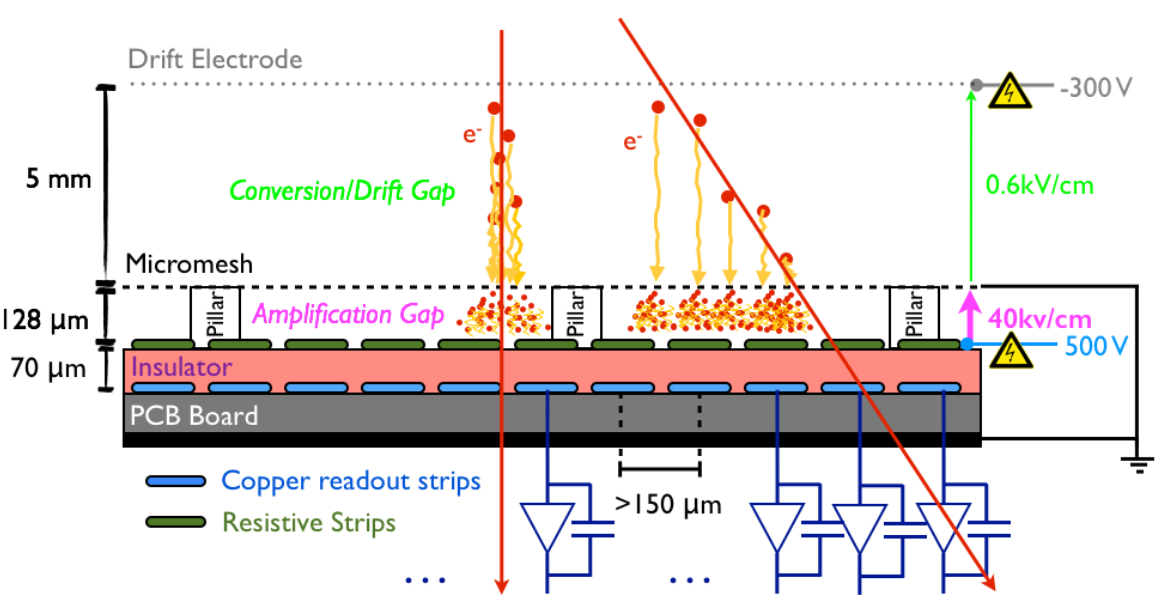
\includegraphics[width=0.75\textwidth]{figures/nsw/nsw_mm_principle}
       % \raisebox{1.12cm}{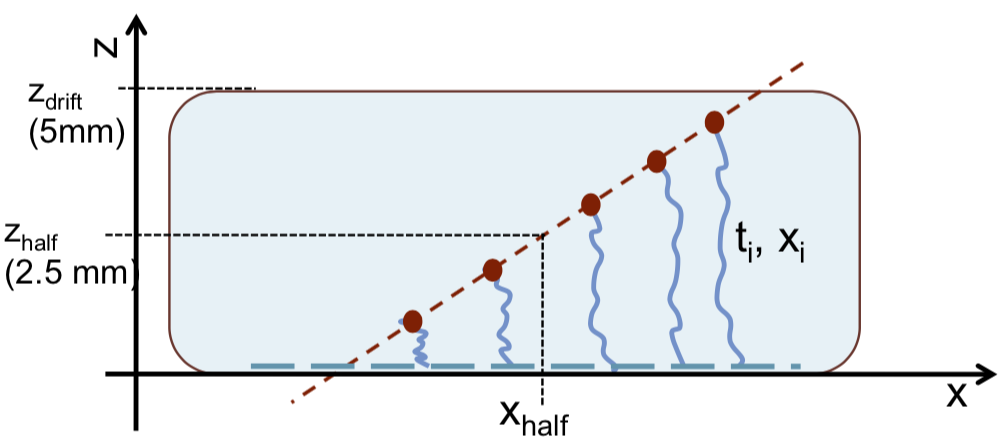
\includegraphics[width=0.37\textwidth]{figures/nsw/mm_tpc_hit_loc}}
        \caption{
        }
        \label{fig:nsw_mm_principle}
    \end{center}
\end{figure}

\begin{figure}[!htb]
    \begin{center}
        %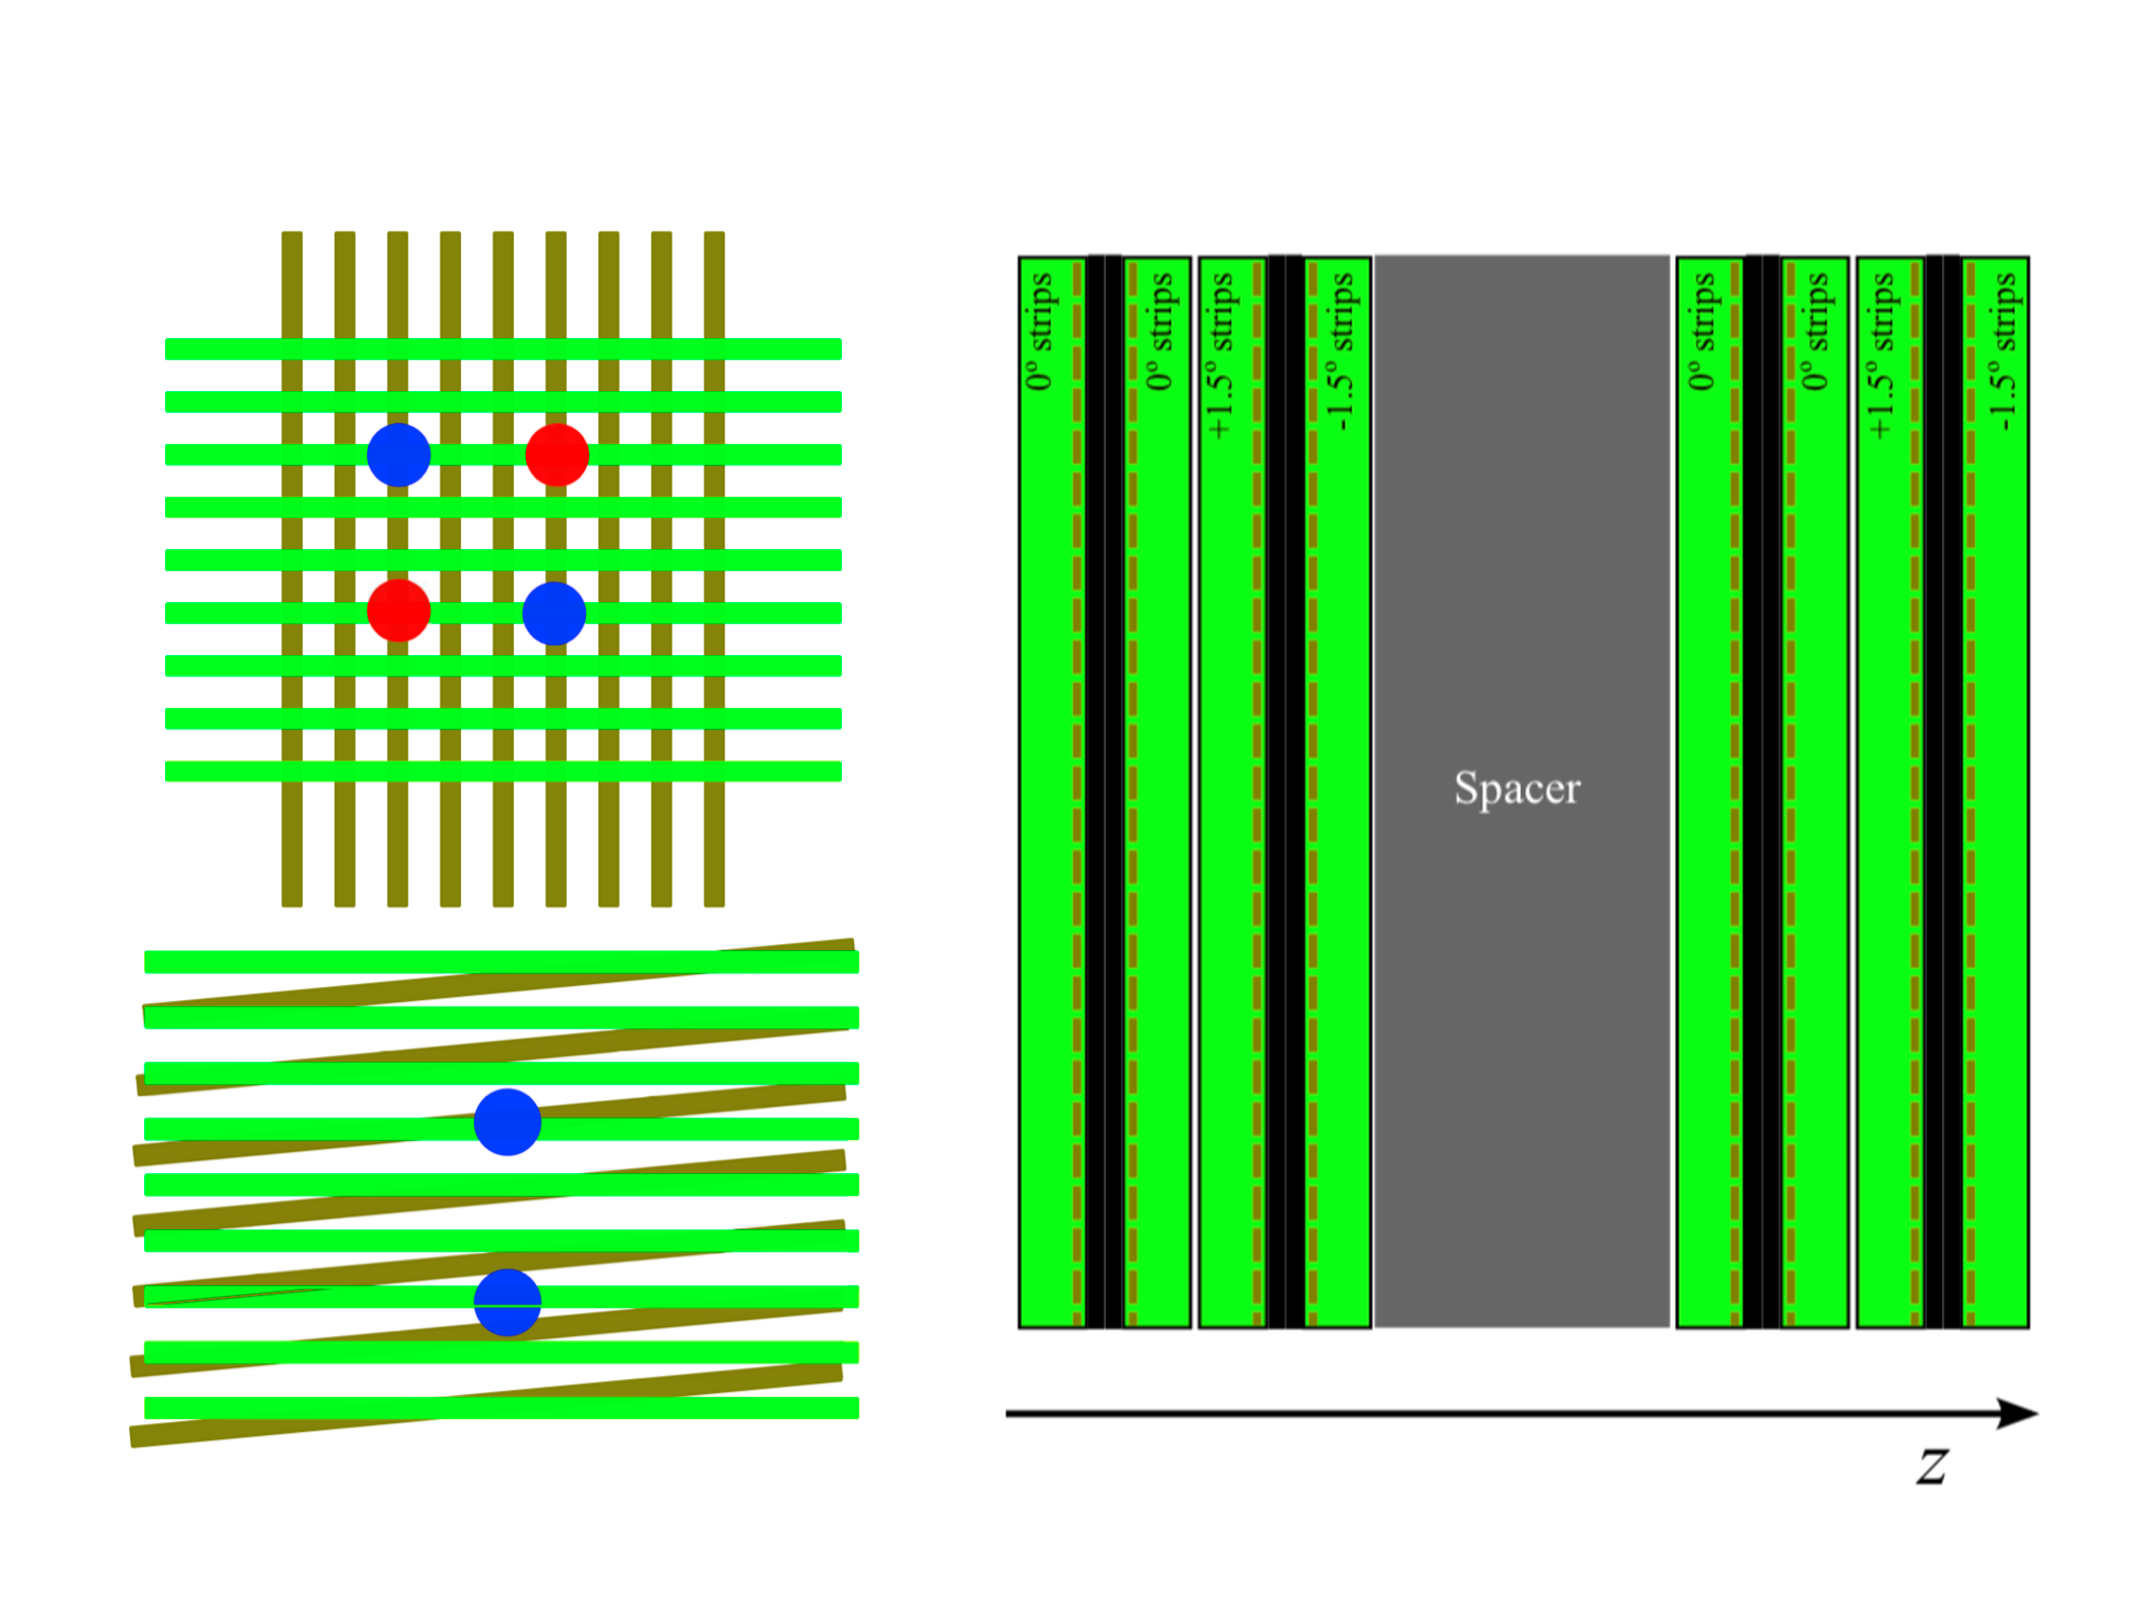
\includegraphics[width=0.8\textwidth]{figures/nsw/mm_ghost_stereoPDF}
        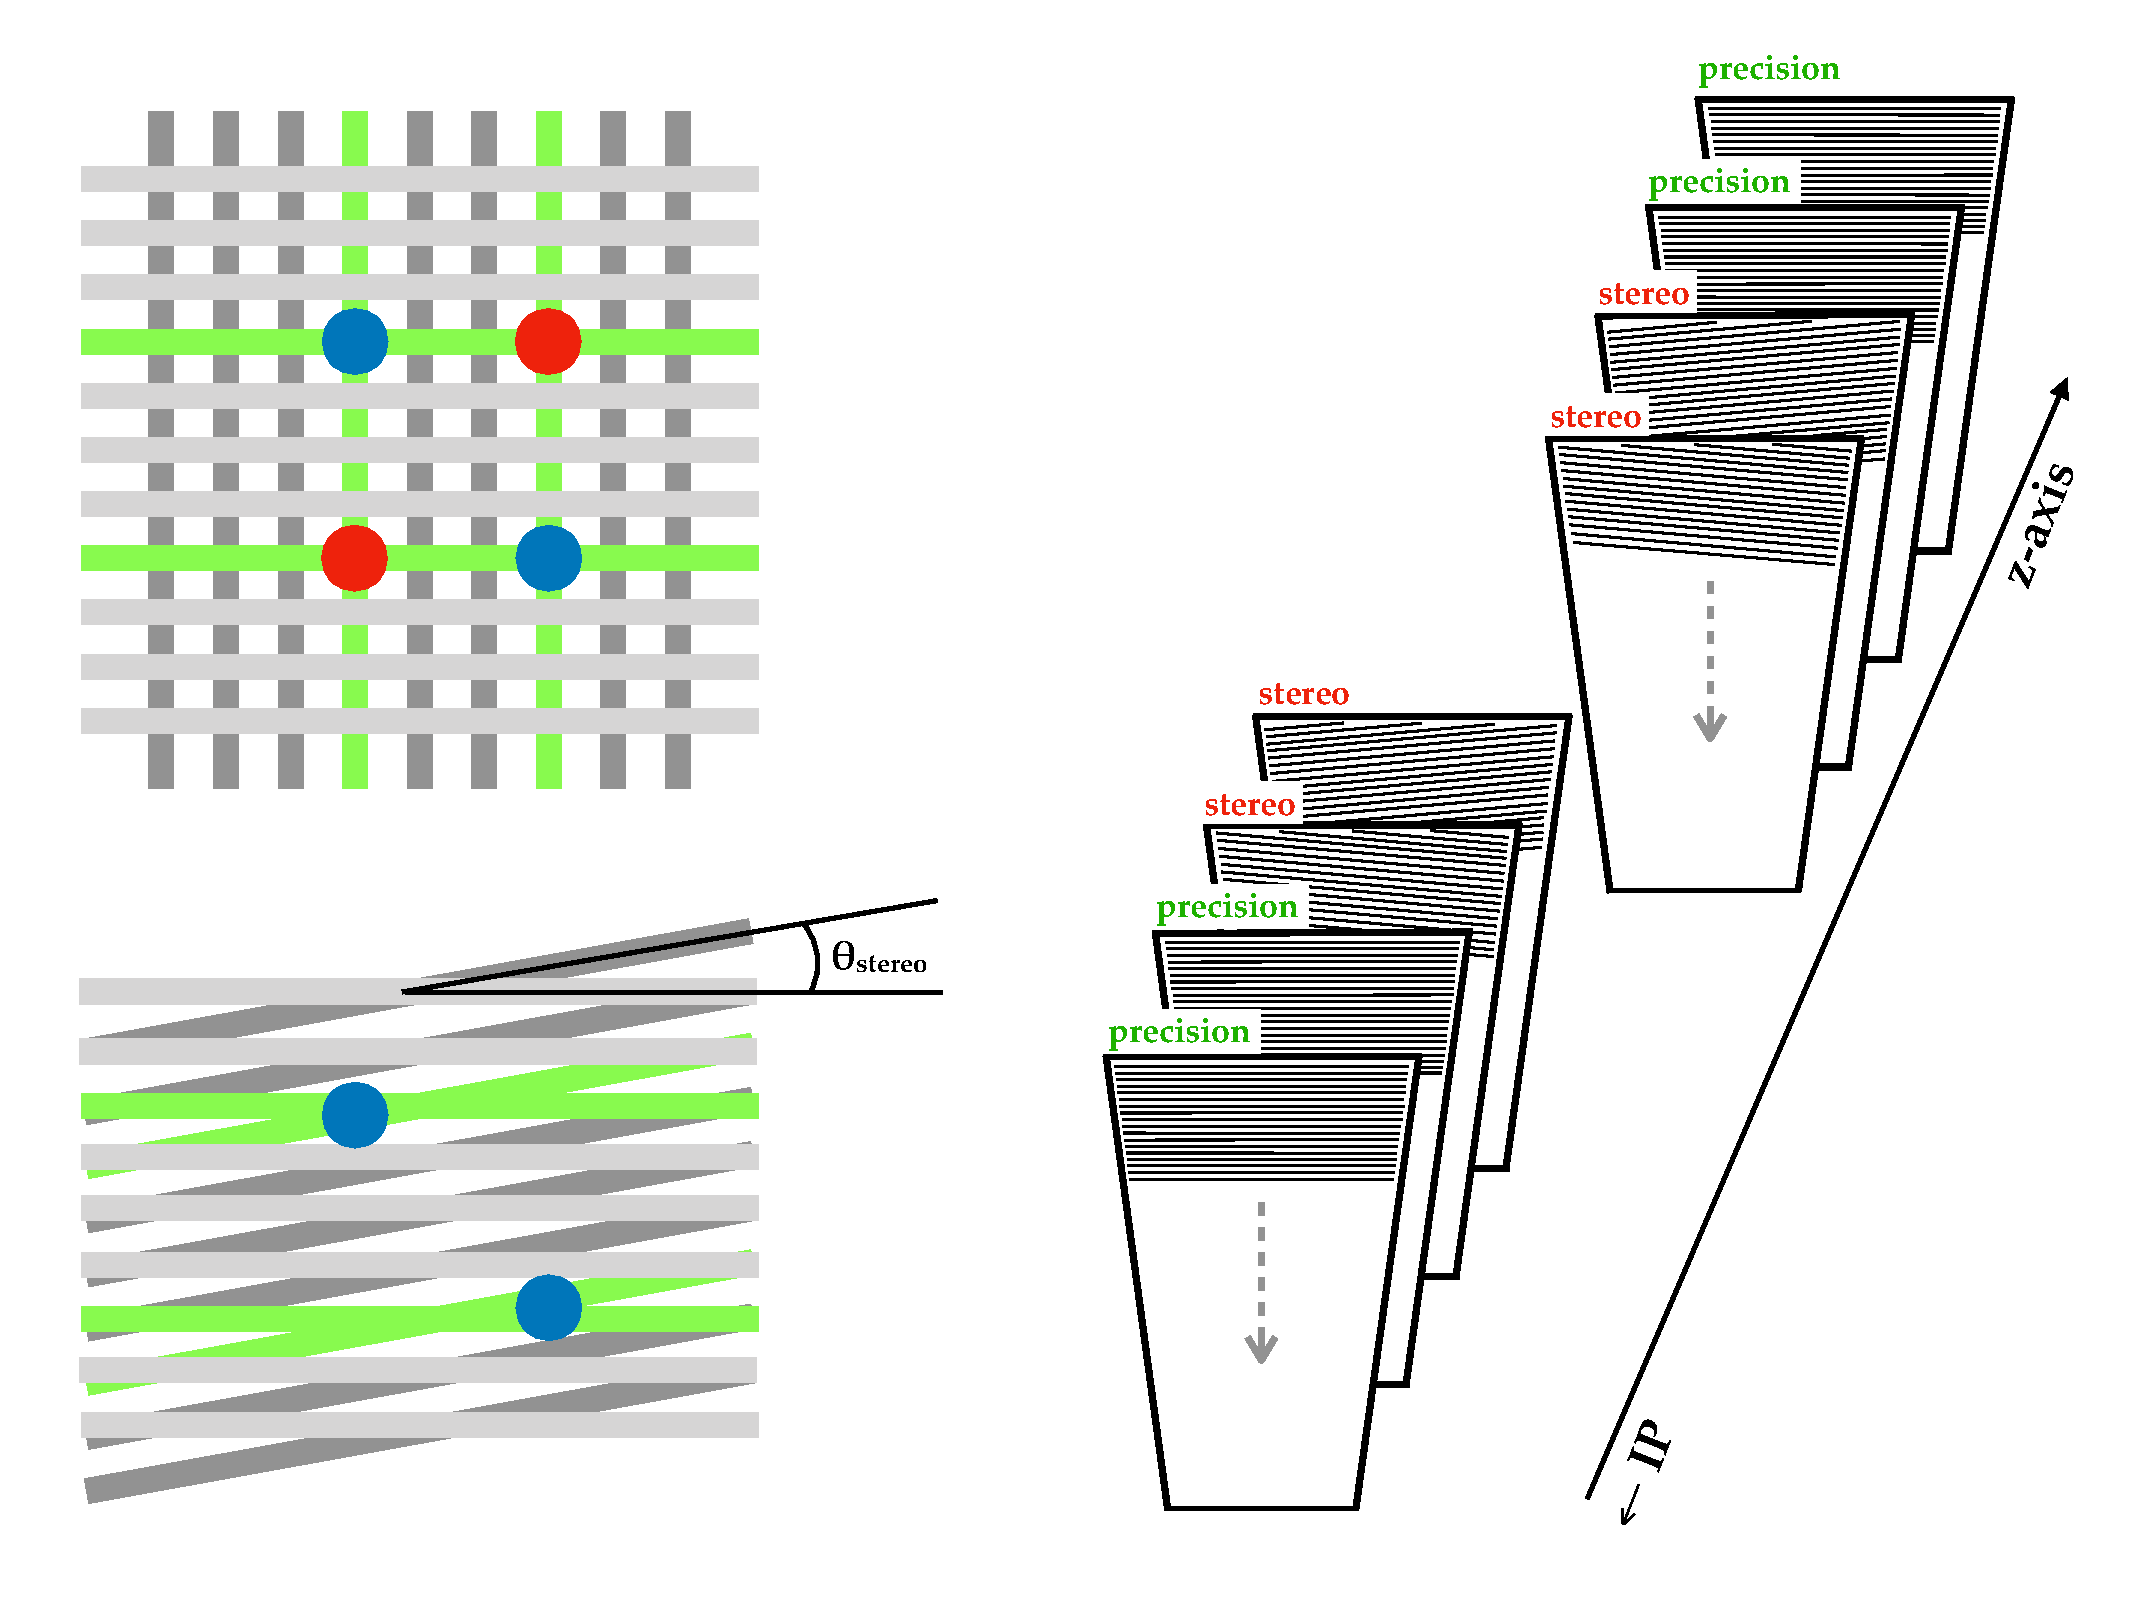
\includegraphics[width=0.8\textwidth]{figures/nsw/mm_stereo_cartoonPDF}
        \caption{
            \textbf{\textit{Left}}: Illustration of the small-angle stereo two-dimensional readout principle.
                The upper panel shows two layers with readout strips perpendicular to each other.
                The lower panel shows two layers with readout strips tilted at a small-angle,
                $\theta_{\text{stereo}}$, relative to one another.
                In both cases, true detector hits are indicated by the blue dots.
                The readout strips registering the hits are indicated in green.
                In the case with perpendicular readout, there are two ghost hits indicated
                by the red dots.
                For perpendicular readout strips, there will generally be $N_{\text{ghost}} = (N^2 - N)$
                ghost hits for $N$ real hits when the readout strips on the two layers have
                equal pitches as in the case of the MM detectors in the NSW.
                On the lower panel, the green readout strips registering the two hits
                do not cross as a result of the small stereo angle and there are no ghost hits.
            \textbf{\textit{Right}}: Illustration of the layout of the `precision' and `stereo'
                readout layers of the two MM quadruplets in a given NSW sector.
                The precision layers, so-called since their readout strips are along $\phi$ and measure directly the
                coordinate in the bending plane of passing muons, are the outer two layers of
                each quadruplet relative to the spacer frame.
                The stereo layers are those with the readout strips tilted at $\pm 1.5^{\degree}$ relative to the precision layers and are the two layers
                in each quadruplet nearest the central spacer frame.
                One stereo layer in each quadruplet has stereo angle $+1.5^{\degree}$ and the other $-1.5^{\degree}$, making
                for $\Delta \theta = 3^{\degree}$ between the two stereo layers.
        }
        \label{fig:mm_stereo}
    \end{center}
\end{figure}

\begin{figure}[!htb]
    \begin{center}
        \raisebox{1.4cm}{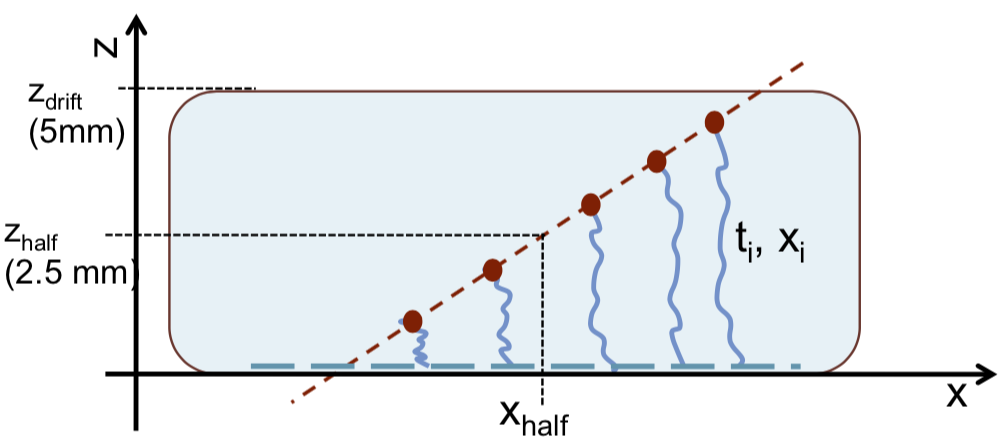
\includegraphics[width=0.48\textwidth]{figures/nsw/mm_tpc_hit_loc}}
        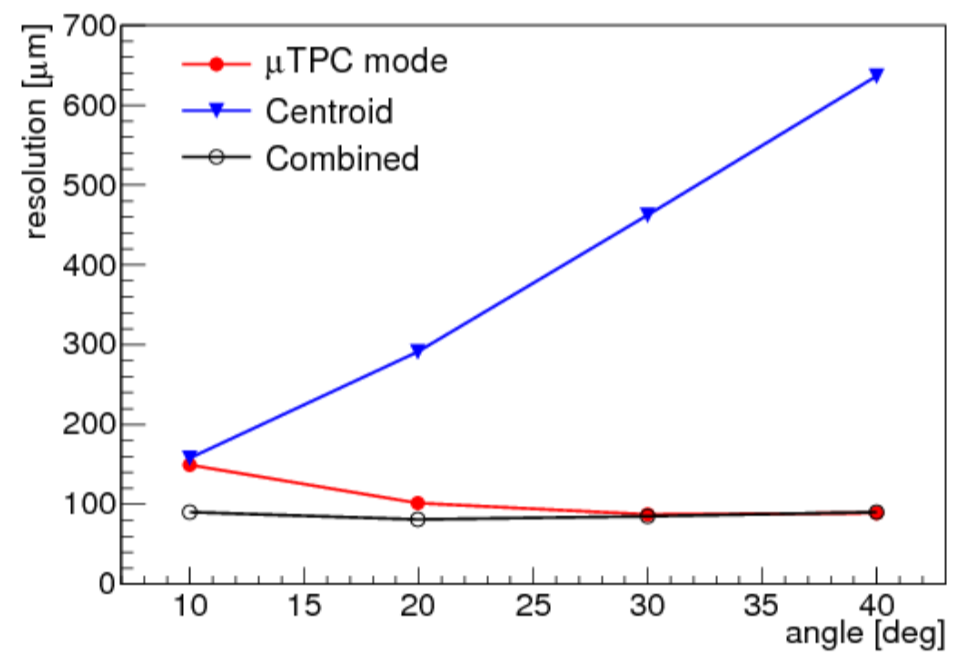
\includegraphics[width=0.48\textwidth]{figures/nsw/tpc_vs_centroid_res}
        \caption{
            \textit{Left}: Illustration of the `$x_{\text{half}}$' method of defining a hit position for
                an inclinded track: the hit position is defined as the position on the readout plane
                corresponding to the half-height location along the reconstructed tracklet in the MM conversion gap.
            \textit{Right}: Expected MM spatial resolution with charge centroid method (blue triangles), $\mu$-TPC
                method (filled red circles), and the combination of the two (black open circles) as a function
                of particle incident angle.
                The combination of the two methods achieves the greater-than $100\,\micron$ single-layer spatial resolution
                required for HL-LHC operation for the expected range of incident angles.
        }
        \label{fig:mm_tpc_hit_loc}
    \end{center}
\end{figure}

%%%%%%%%%%%%%%%%%%%%%%%%%%%%%%%%%%%%%%%%%%%%%%%%%%%%%%%%%%%%%%%
% STGC
%%%%%%%%%%%%%%%%%%%%%%%%%%%%%%%%%%%%%%%%%%%%%%%%%%%%%%%%%%%%%%%
\subsection{The Small-strip Thin Gap Chamber Detectors}
\label{sec:nsw_stgc}

The sTGC are those detectors stated as being primarily used for producing trigger primitives
to be used by the Level-1 muon trigger system.
As triggering detectors, they have fast signal formation and readout times owing to their characteristic high
operating electric fields.
This enables
them to provide accurate bunch crossing identification (i.e. assigning hits to a specific bunch crossing).
The average drift time of ionisation electrons within the sTGC chambers is less than 25\,ns,
with the earliest cluster arrival times well below 10\,ns.
Figure~\ref{fig:stgc_timing} shows the distribution of the measured drift times in an
sTGC, with 95\% of the measured and simulated data being inside a 25\,ns (the LHC bunch crossing
frequency) time window.
The sTCG detectors also provide good online angular resolution --- better than 1\,mrad --- for the track segments
reconstructed across the layers of an sTGC quadruplet, meaning fairly good spatial resolution.
The high quality angular resolution allows for good \pT~determination based on the trigger primitives
provided to the Level-1 trigger.
Offline spatial reconstruction for track segments provided by the sTGC detectors will also be good, matching
the sub-100$\,\micron$ threshold for the HL-LHC precision tracking requirements in the forward region
of the muon system.

\begin{figure}[!htb]
    \begin{center}
        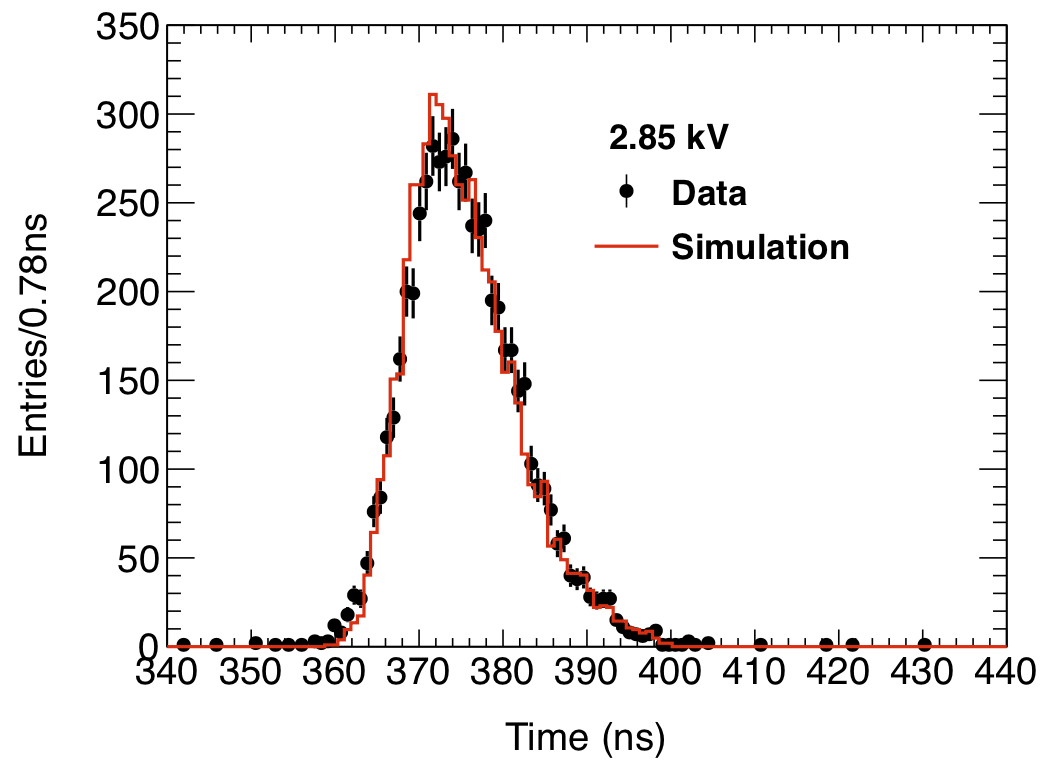
\includegraphics[width=0.5\textwidth]{figures/nsw/stgc_timing}
        \caption{
            Due to the very thin gap and the intense electric field applied,
            $\approx95$\,\% of the measured drift times of passing MIPs are
            confined within a window of 25\,ns, showing that the sTGC
            are capable of relaible bunch crossing assignment.
        }
        \label{fig:stgc_timing}
    \end{center}
\end{figure}

The basic sTGC detector is shown in Figure~\ref{fig:stgc_drawing}.
It consists of a grid of $50\,\micron$ gold-plated tungsten wires with $1.8$\,mm pitch
sandwiched between two cathode planes at a distance of $1.4$\,mm.
On one plane there are the readout pads and on the other the strips.
The strips have a $3.2$\,mm pitch, which is smaller than that of the current TGC
detectors used in the current forward muon system (Figure~\ref{fig:muon_plan_view_eta}),
which is the origin of the name of the sTGC detectors.
The wires and strips are perpendicular, with the wires stretching along $r$ and the
strips along $\phi$.

The pads are used to form coincidences between the layers of the sTGC quadruplets in order
to form projective trigger primitives corresponding to muon tracks pointing roughly back to the IP.
There are $\approx 1300$ pads per sTGC layer.
The collected charge from all components of the sTGC --- the pads, strips, and wires --- associated with a traversing particle are read out and
used for the subsequent offline precision muon-track reconstruction.
Two-dimensional readout is achieved by the $r$ and $\phi$ information provided by the strips
and wires, respectively.
To help cope with the foreseen high particle rates, and to reduce the types of tracking ambiguities
described in Section~\ref{sec:nsw_mm} due to combinatorial hits, only
those wires and strips covering the projective area of pads registering the passage of
the particle are read out.
Additionally, wires are grouped together (i.e. multiple wires correspond to a single readout
channel) as only a rough measurement of the azimuthal coordinate --- not relevant for \pT~determination in the trigger---
is needed.
With the charge information collected from the three sub-components, the sTGC is able to achieve very
good spatial resolutions approaching $approx 80\,\micron$ ($\approx 100\,\micron$) per layer for perpendicular (inclined) tracks.

\begin{figure}[!htb]
    \begin{center}
        \raisebox{0.8cm}{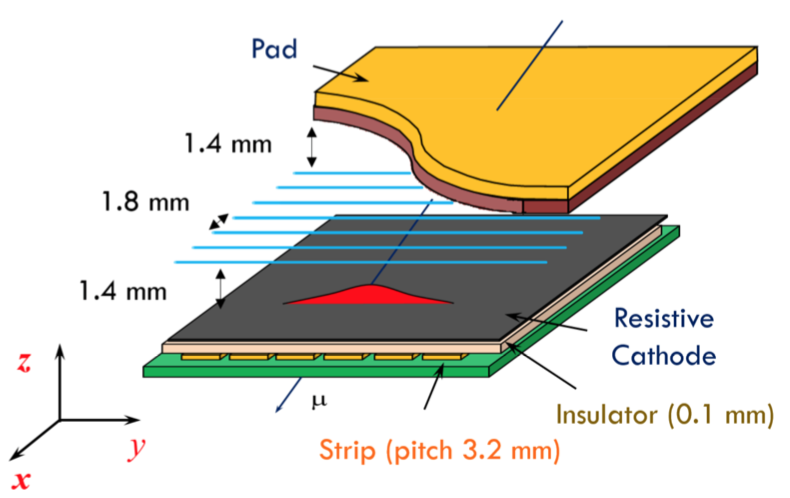
\includegraphics[width=0.52\textwidth]{figures/nsw/stgc_drawing}}
        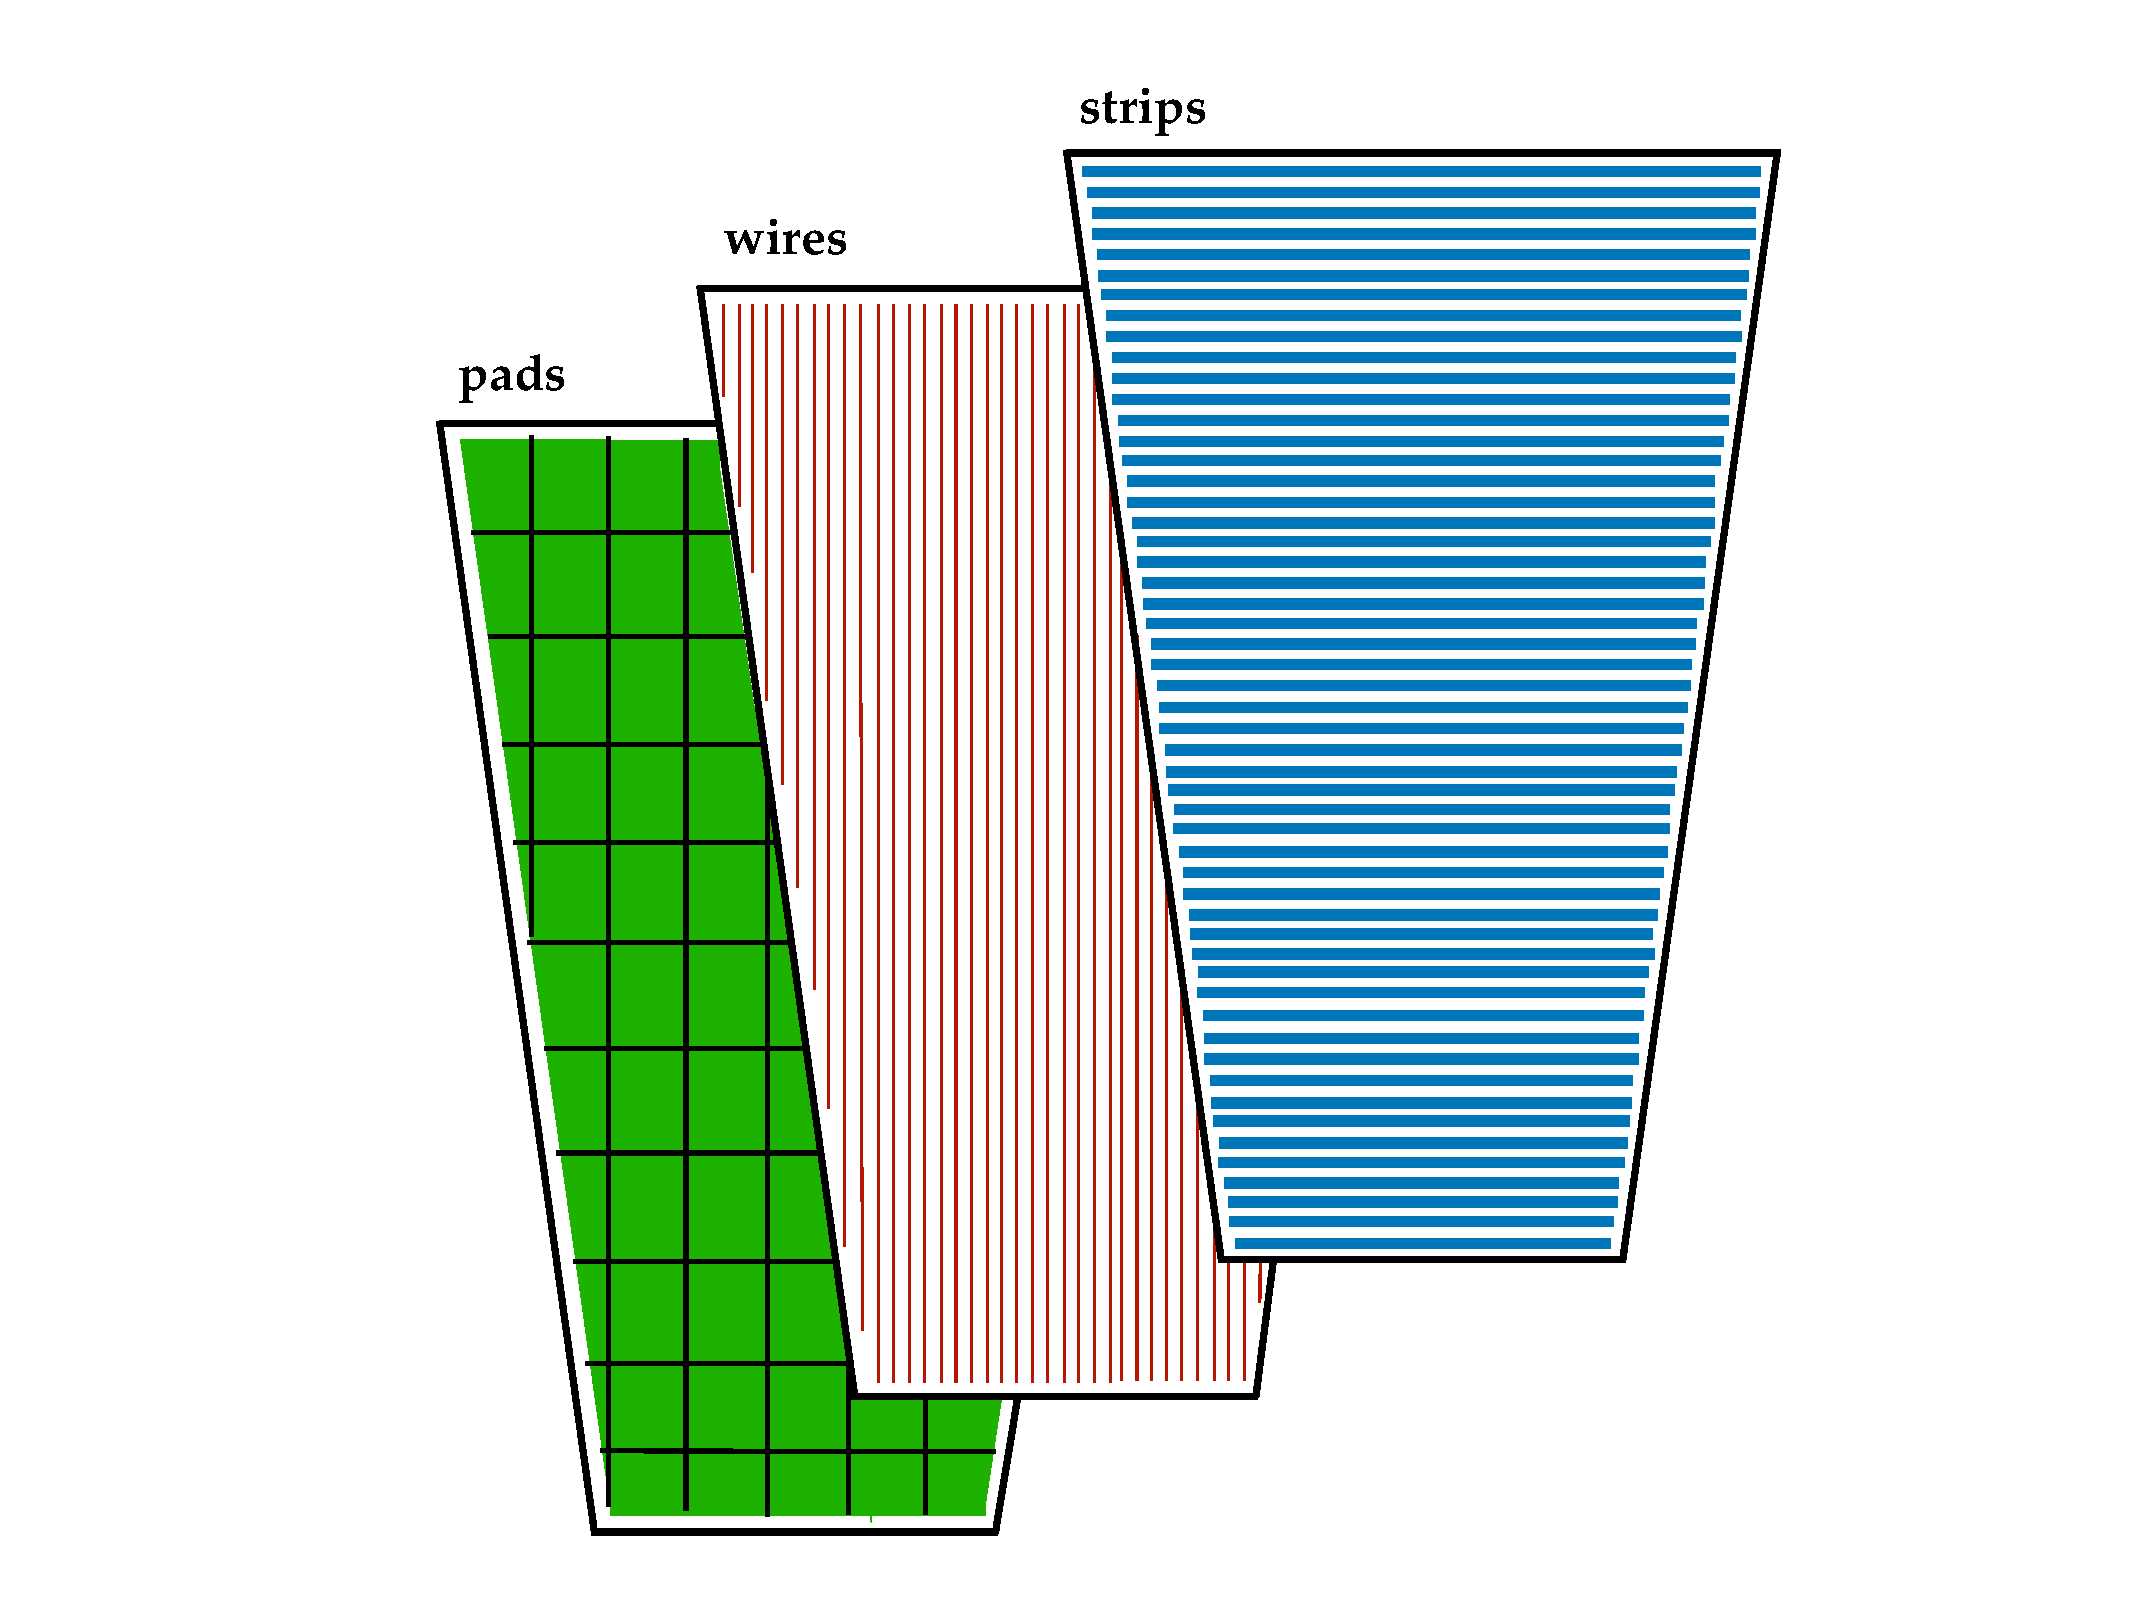
\includegraphics[width=0.45\textwidth]{figures/nsw/stgc_layer_cartoonPDF}
        \caption{
            \textbf{\textit{Left}}: Graphical representation of the internal structure of an
                sTGC detector.
                The passage of a traversing MIP (black line) induces signals on the anode wires, readout pads,
                and strips behind the resistive cathode planes as a result of the drifting of ionisation
                charges and their subsequent multiplication (in red).
            \textbf{\textit{Right}}: Illustration of the geometry of the sTGC pads, wires, and strips and their
                relative layout in a single sTGC layer.
                The strips (blue) are along $\phi$ and provide the measurement of the precision momentum coordinate
                in the particle bending plane.
                The wires are along $r$ and provide measurements sensitive to $\phi$.
                The pads provide information necessary for building trigger coincidences between
                the layers of an sTGC quadruplet and determine which subset of wires and strips will
                subsequently be readout upon a Level-1 trigger accept.
                The drawing is not to scale and does not illustrate the actual segmentation
                of the readout components in a given layer, only their relative orientation.
        }
        \label{fig:stgc_drawing}
    \end{center}
\end{figure}

\FloatBarrier

%%%%%%%%%%%%%%%%%%%%%%%%%%%%%%%%%%%%%%%%%%%%%%%%%%%%%%%%%%%%%%%%%%%%%%%
% NSW ELX
%%%%%%%%%%%%%%%%%%%%%%%%%%%%%%%%%%%%%%%%%%%%%%%%%%%%%%%%%%%%%%%%%%%%%%%
\section{NSW Readout Electronics and Detector Instrumentation}
\label{sec:nsw_elx}

{\color{make it clearer that the tracking data readout of both sTGC and MM is very similar, since they
both use the VMM...?}}

To a very large extent, high-performance detectors are realised and made
possible only by their interfacing to equally high-performance readout electronics;
that is, high quality electronics enable high quality detectors.
{\color{red}{See Appendix XXX for a discussion on the general characteristics of
detector readout electronics.}}
In this section, therefore, an introduction to the frontend electronics\footnote{`Frontend' electronics
are those housed directly on the detectors themselves and are responsible for reading out the
detector signals and potentially many other responsibilities, such as calibration, configuration, and
detector controls (temperature monitoring, etc...). `Backend' electronics refer to those
not necessarily located in the experimental cavern housing the detectors but are in the nearby
service areas or on the surface (c.f. Figu:e~\ref{fig:p1}) and are dedicated, for example, to the implementation of detector trigger logic
and data decoding and event building (i.e. gathering all data from detector hits associated with a given event).}
relevant to the NSW will be given.
There is a large set of both frontend and backend electronics specifically
designed and constructed for the NSW~\cite{NSWFrontEndChristos}.
Here, though, we will focus primarily on the frontend electronics.
The NSW frontend electronics revolve around the operation of a family
of rather complex application specific integrated circuits (ASICs),
each targetting a specific (set of) purpose(s) related to data-acquisition or
constructing trigger primitives:
%including a family of application specific integrated circuits (ASICs):

\begin{description}
    \item[] \textbf{VMM}~\cite{VMM1GDG,VMMASIC,VMM3George} Frontend readout ASIC used for precision and fast trigger data signal collection in both MM and sTGC detectors
    \item[] \textbf{ROC}~\cite{NSWTDR,NSWFrontEndChristos} `ReadOut Controller' ASIC, responsible for buffering and aggregating precision data from the VMM
    \item[] \textbf{TDS}~\cite{TDS} `Trigger Data Serialiser' ASIC, processes trigger signals from VMMs on the sTGC detectors and prepares trigger primitives for the NSW Level-1 muon trigger logic
    \item[] \textbf{ART}~\cite{NSWTDR,ARTASIC} 'Address in Real Time' ASIC, processes trigger signals from VMMs on the MM detectors and prepares trigger primitives for the NSW Level-1 muon trigger logic
\end{description}

The VMM ASIC is the primary ASIC of the NSW: all other ASICs listed above take as input
the outputs of the VMM and, in this respect, are secondary.
The work of the current author on the NSW frontend electronics is based almost exclusively
on the characterisation and validation of the VMM ASIC.
For these reasons, focus will be given on describing the VMM in Section~\ref{sec:vmm}.
For the interested reader, further information on the ROC, TDS, and ART ASICs is
provided in the references above.
The interface of the NSW frontend electronics to the associated detectors is dictated for the most part
by the geometry, type, and number of the detectors' readout elements (MM: strips, sTGC: strips, wires, and pads)
and foreseen space limitations in the ATLAS detector.
The work in the present thesis concerns the frontend boards related to the MM detectors.
This is mainly due to the fact that the VMM was initially conceptualised as a frontend ASIC specialised
for MPGD detectors and its initial prototypes were studied under this context by the RD51 collaboration
at CERN which is devoted to the development of MPGD technologies, such as the MM detectors.\footnote{For more information
on the RD51 collaboration, visit their homepage: \url{http://rd51-public.web.cern.ch/rd51-public/}.}
In Section~\ref{sec:nsw_boards}, then, a description of the relevant front-end boards used in the
study, validation, and integration of the VMM ASIC, as well as those that will be used in
the MM detectors of the NSW, will be given.
The analgogous VMM-based frontend boards for the sTGC detectors are objectively more complicated than those
of the MM detectors for purely technical and uninteresting reasons.
Their description can be found elsewhere~\cite{NSWTDR}.
{\color{red}{Maybe change how I describe why I am focused on MM detectors etc...}}

\subsection{The VMM ASIC}
\label{sec:vmm}

The VMM is a custom ASIC that can be used in a variety of charge-interpolated tracking
detectors.
There have been several iterations of the VMM over the years, starting with the VMM1~\cite{VMM1GDG} and
moving up to the VMM3~\cite{VMMASIC,VMM3George}.
An illustration of the evolution of complexity of the VMM ASIC is shown in Figure~\ref{fig:vmms_silicon}.
The VMM1 was a purely analog readout ASIC considered to be a prototype of the initial VMM functionalities.
The VMM2 was an extensive upgrade of the VMM1, adding the necessary digital logic and functional blocks
required for the NSW detectors.
The VMM3 is the final version of the ASIC\footnote{In actuality, there have been two versions of the
VMM3: the VMM3 and the `VMM3a'. The VMM3a is the true final version that will be used in the NSW
and addresses issues found during the testing and validation of the first round of the VMM3 production}
providing enhanced functionality required for data taking in ATLAS
as well as addressing bugs found in the operation of the VMM2
VMM3 is the version that will be used
in the NSW once installed in ATLAS.
The VMM implements all logic using triple modular redundancy (TMR) to protect itself
from single event upsets (SEUs) that are expected to be quite common in the
harsh radiation environments in which the NSW will be situated.

The VMM is composed of 64 discrete frontend channels, each to be connected to a detector
readout element.
A block diagram illustrating the functional blocks of the VMM3 and its channels is
shown in Figure~\ref{fig:vmm3_channel}.
Each channel has a dedicated charge amplifier (`CA' in Figure~\ref{fig:vmm3_channel}) and signal
shaping functionality,
threshold discriminator, test-pulse injection capacitor with adjustable amplitude provided
by a 10-bit digital-to-analog converter (DAC), and precise signal amplitude and timing measurements digitally readout via
internal per-channel analog-to-digital converters (ADCs).
The amplitude measurement of the input pulse is digitised by a 10-bit ADC (`PDO', for `peak detector output', in Figure~\ref{fig:vmm3_channel})
and the timing estimation of the signal pulse's peak is digitised by an 8-bit ADC (`TDO', for `time detector output', in Figure~\ref{fig:vmm3_channel}).
The digitised output of these amplitude and timing measurements are calculated by these
internal ADCs within 200\,ns and stored in internal buffers of the VMM.
The buffered data is stored until selected for readout by another ASIC housed on the same frontend
board as the VMM, the ROC, based on the buffered data's bunch crossing.
The PDO and TDO data are those used in the precision hit reconstruction in the detectors.
The hit timing information provided by the TDO is critical only for the MM detectors which
rely primarily on the $\mu$-TPC hit reconstruction method, as illustrated in Figure~\ref{fig:mm_tpc_hit_loc} (right).
For the sTGC, the accurate timing information is not required for precision tracking and,
to increase readout bandwidth, the timing information will likely not be serialised
in the data output from the sTGC frontend electronics.
%{\color{red}{For the precision hit reconstruction, the timing information is critical only for the MM
%detectors which rely on the $\mu$-TPC hit reconstruction method which requires
%precision time measurements for building the tracklets within the drift region of the
%MM detector. For the sTGC the accurate timing information is not required
%for precision tracking and, to increase readout bandwidth, the timing information will not be
%serialised.}}

In addition to the precision data useful for reconstructing high-level muon tracks provided by
the PDO and TDO measurements, the VMM can also operate at a faster mode used for
providing data needed for the building of trigger primitives.
In the trigger mode referred to as the `Address-in-Real-Time' (ART) mode,
the VMM outputs the \textit{first} channel address (i.e. MM strip number) on which
an above-threshold peak was detected.
An alternative trigger mode relies on the VMM's ability to perform a fast digitisation of
the signal pulse amplitude using a 6-bit ADC, providing a coarse but rapid measurement
of the signal amplitude.
Additionally, the VMM can output fast timing signals, such as a flag indicating a signal over threshold (`Time-Over-Threshold', or TOT as in Figure~\ref{fig:vmm3_channel}).
The ART trigger scheme is used for the MM trigger primitives and the combination
of the coarse 6-bit amplitude and fast-timing signals is used for building the
sTGC trigger primitives.

One of the powers of the VMM is its highly configurable nature.
This, of course, makes the ASIC quite complex in terms of its design but is
advantageous in terms of its range usefulness.
Some of the main configurable items are the peaking (integration) time of the signal shaper
(25, 50, 100, and 200\,ns), adjustable thresholds per-VMM configured by an on-VMM
10-bit (DAC),
adjustable channel gains (0.5, 1, 3, 4.5, 6, 9, 12, and 16\,mV/fC),
time-to-amplitude conversion (TAC) ramp time (60, 100, 350, and 650\,ns) relevant for the timing measurements,
and channel threshold trimmers provided by 5-bit DACs that adjust each channel's individual
threshold around the globally-configured (per-VMM) threshold.
The VMM input can also be configured to handle either positive or negative input
signals.
This latter fact is necessary for the NSW, in which the sTGC and MM detectors
will induce signals of opposite polarity on their readout elements.\footnote{The MM strips and
sTGC wires produce signals of opposite polarity as the sTGC strips and pads.}

\begin{figure}[!htb]
    \begin{center}
        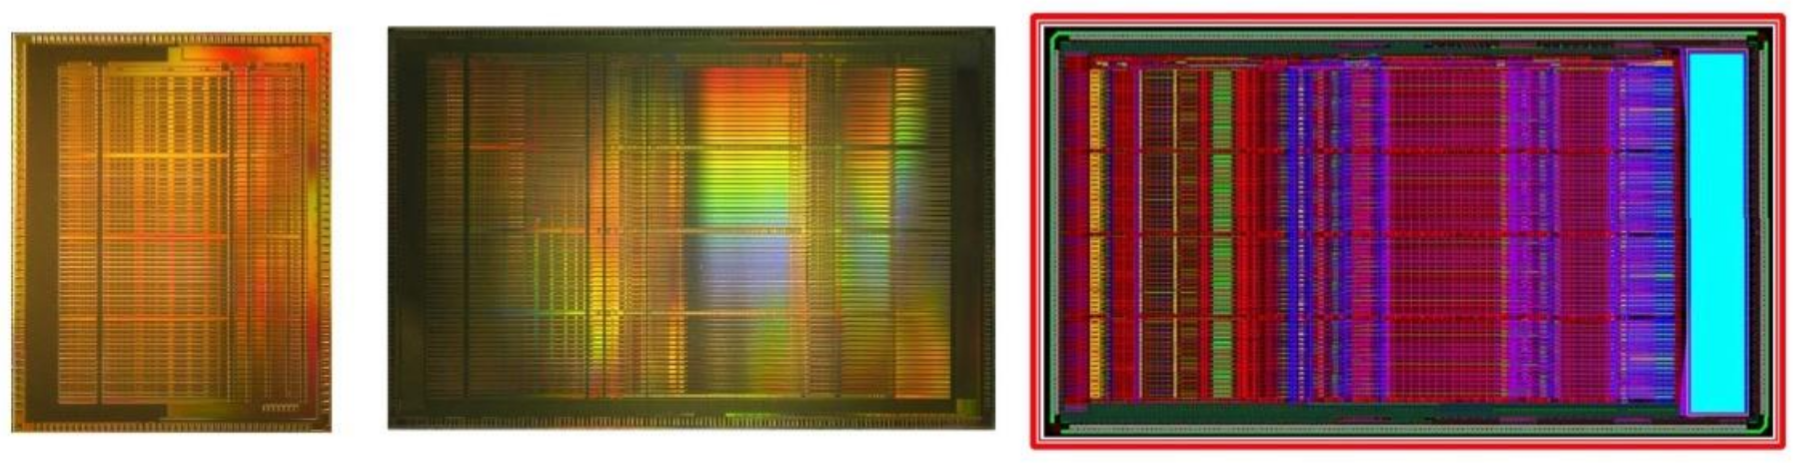
\includegraphics[width=0.8\textwidth]{figures/nsw/vmm/vmms_silicon}
        \caption{
            Evolution of the VMM ASIC.
            Shown are the silicon dies or routing of the the VMM1 (\textbf{\textit{left}}), to the VMM2 (\textbf{\textit{middle}}), and 
            the VMM3 (\textbf{\textit{right}}), the final version that will be used in the NSW.
            The VMM1 has an area of 50\,mm$^2$ with $\approx 500$\,k MOSFETs, the VMM2 area is 115\,mm$^2$ with $>5$\,M MOSFETs,
            and the VMM3 area is 130\,mm$^2$ with $>6$\,M MOSFETs.\protect\footnotemark%
        }
        \label{fig:vmms_silicon}
    \end{center}
\end{figure}
\footnotetext{`MOSFET' stands for metal-oxide-semiconductor field-effect  transistor', the most widely used transistor in digital and analog electronics.}

\begin{figure}[!htb]
    \begin{center}
        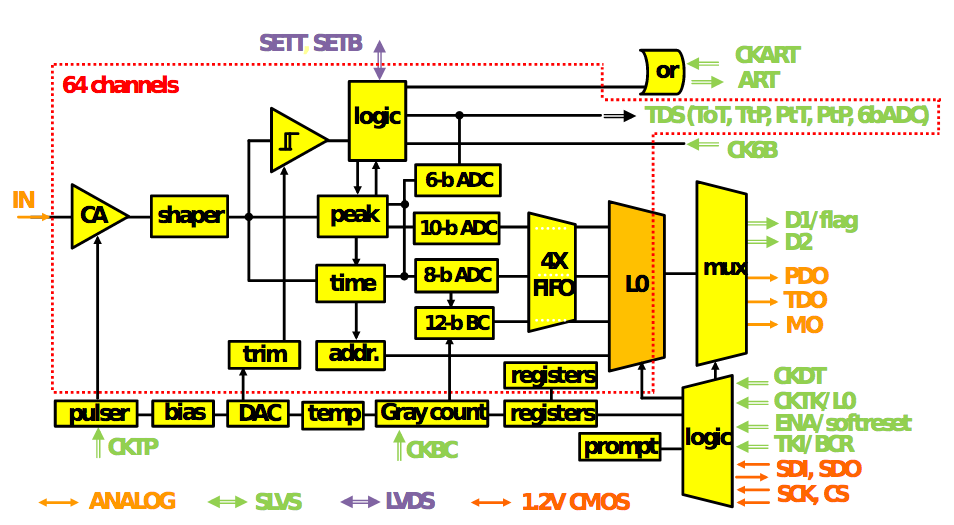
\includegraphics[width=0.8\textwidth]{figures/nsw/vmm/vmm3_channel}
        \caption{
            Architecture of the VMM3.
            The items contained within the dotted red line are repeated
            for each of the 64 channels of the VMM.
        }
        \label{fig:vmm3_channel}
    \end{center}
\end{figure}

\subsection{Frontend-electronics Boards for the NSW}
\label{sec:nsw_boards}

There have been two classes of frontend boards encountered
throughout the work on the NSW electronics represented in this thesis.
The first class relates to a type of frontend board that is not specific to the NSW
but which houses one (or several) VMM ASICs.
The second class relates to prototype frontend boards following the design to be used
in the NSW to readout the MM detectors, the so-called MMFE8 frontend board.
Figure~\ref{fig:frontend_boards} provides pictures of these two classes of frontend
boards with relevant parts indicated.

The general purpose frontend boards, such as the GPVMM in Figure~\ref{fig:frontend_boards}, are those used primarily for the direct study
and characterisation of the VMM ASIC.
The prototype MMFE8 frontend boards allow for a more realistic interface to the MM
detectors to be studied as well as for the overall design and layout of the hardware components on the
boards themselves to be studied and optimised.
One such optimisation was the placement of the DC-to-DC converters used for the on-board power distribution.\footnote{In the
final MMFE8 prototype frontend boards, and in those to be used in the NSW,
the DC-to-DC converters are packaged in the so-called FEAST ASIC developed by CERN.
Further information at \url{https://project-dcdc.web.cern.ch/project-dcdc/Default.html}}
DC-to-DC converters are potential sources of electronic noise and stray electromagnetic fields as a result of
their high switching frequencies.
When placed directly on the frontend boards, their nearness to the noise-sensitive readout
elements means that the matter of their placement and shielding needs to be handled carefully.

The types of boards discussed here have allowed for the study of the VMM ASIC both on- and off-detector,
where in the latter case prototype MM detectors were used ({\color{red}{More to say in Section XXX}}).
Over the timespan of the present thesis, many iterations of each type of frontend board
were encountered, with subsequent iterations adapting to the evolution of the VMM, for example (Figure~\ref{fig:vmms_silicon}).
In addition to housing the VMM ASIC, the frontend boards house a
\textsc{Xilinx} field-programmable gate array (FPGA). 
One of the main purposes of the FPGA is to aggregate the data being output from the VMM
and prepare it for being sent off-board via standard network protocols over Ethernet to the
backend data-acquisition system ({\color{red}{Section XXX}}).
Additionally, the FPGA responds to commands and requests submitted by users via the software
interface ({\color{red}{Section XXX}}).
Such commands may have as endpoint the FPGA itself or they may require the FPGA to forward
them to the VMM ASIC.
%may have as end and either adjusts its own configuration parameters or
%forwards the commands to the VMM such that it itself may respond.

The GPVMM board has a simple connector designed in such a way that lends itself to
be easily adapted to many types of detectors in labs and teststands.
The MMFE8 board, both the prototypes and those to be used in the NSW, use a ZEBRA\footnote{More information
on ZEBRA-type connectors can be found online at \url{https://en.wikipedia.org/wiki/Elastomeric_connector}} elastomeric
connector that allows for a seamless interconnect between the readout strips on the MM detector layers
and the VMM channel inputs.
The principle of the ZEBRA connector is illustrated in Figure~\ref{fig:zebra_connector}.
%In the final version of the MMFE8 frontend board to be used for interfacing with the MM detectors,
%the Ethernet readout will be replaced b
%the role of the FPGA will be replaced by the combination of the ROC ASIC, mentioned in the previous section,
%and the CERN-provided Slow Control Adapter (SCA) ASIC~\cite{GBTASIC}

\begin{figure}[!htb]
    \begin{center}
        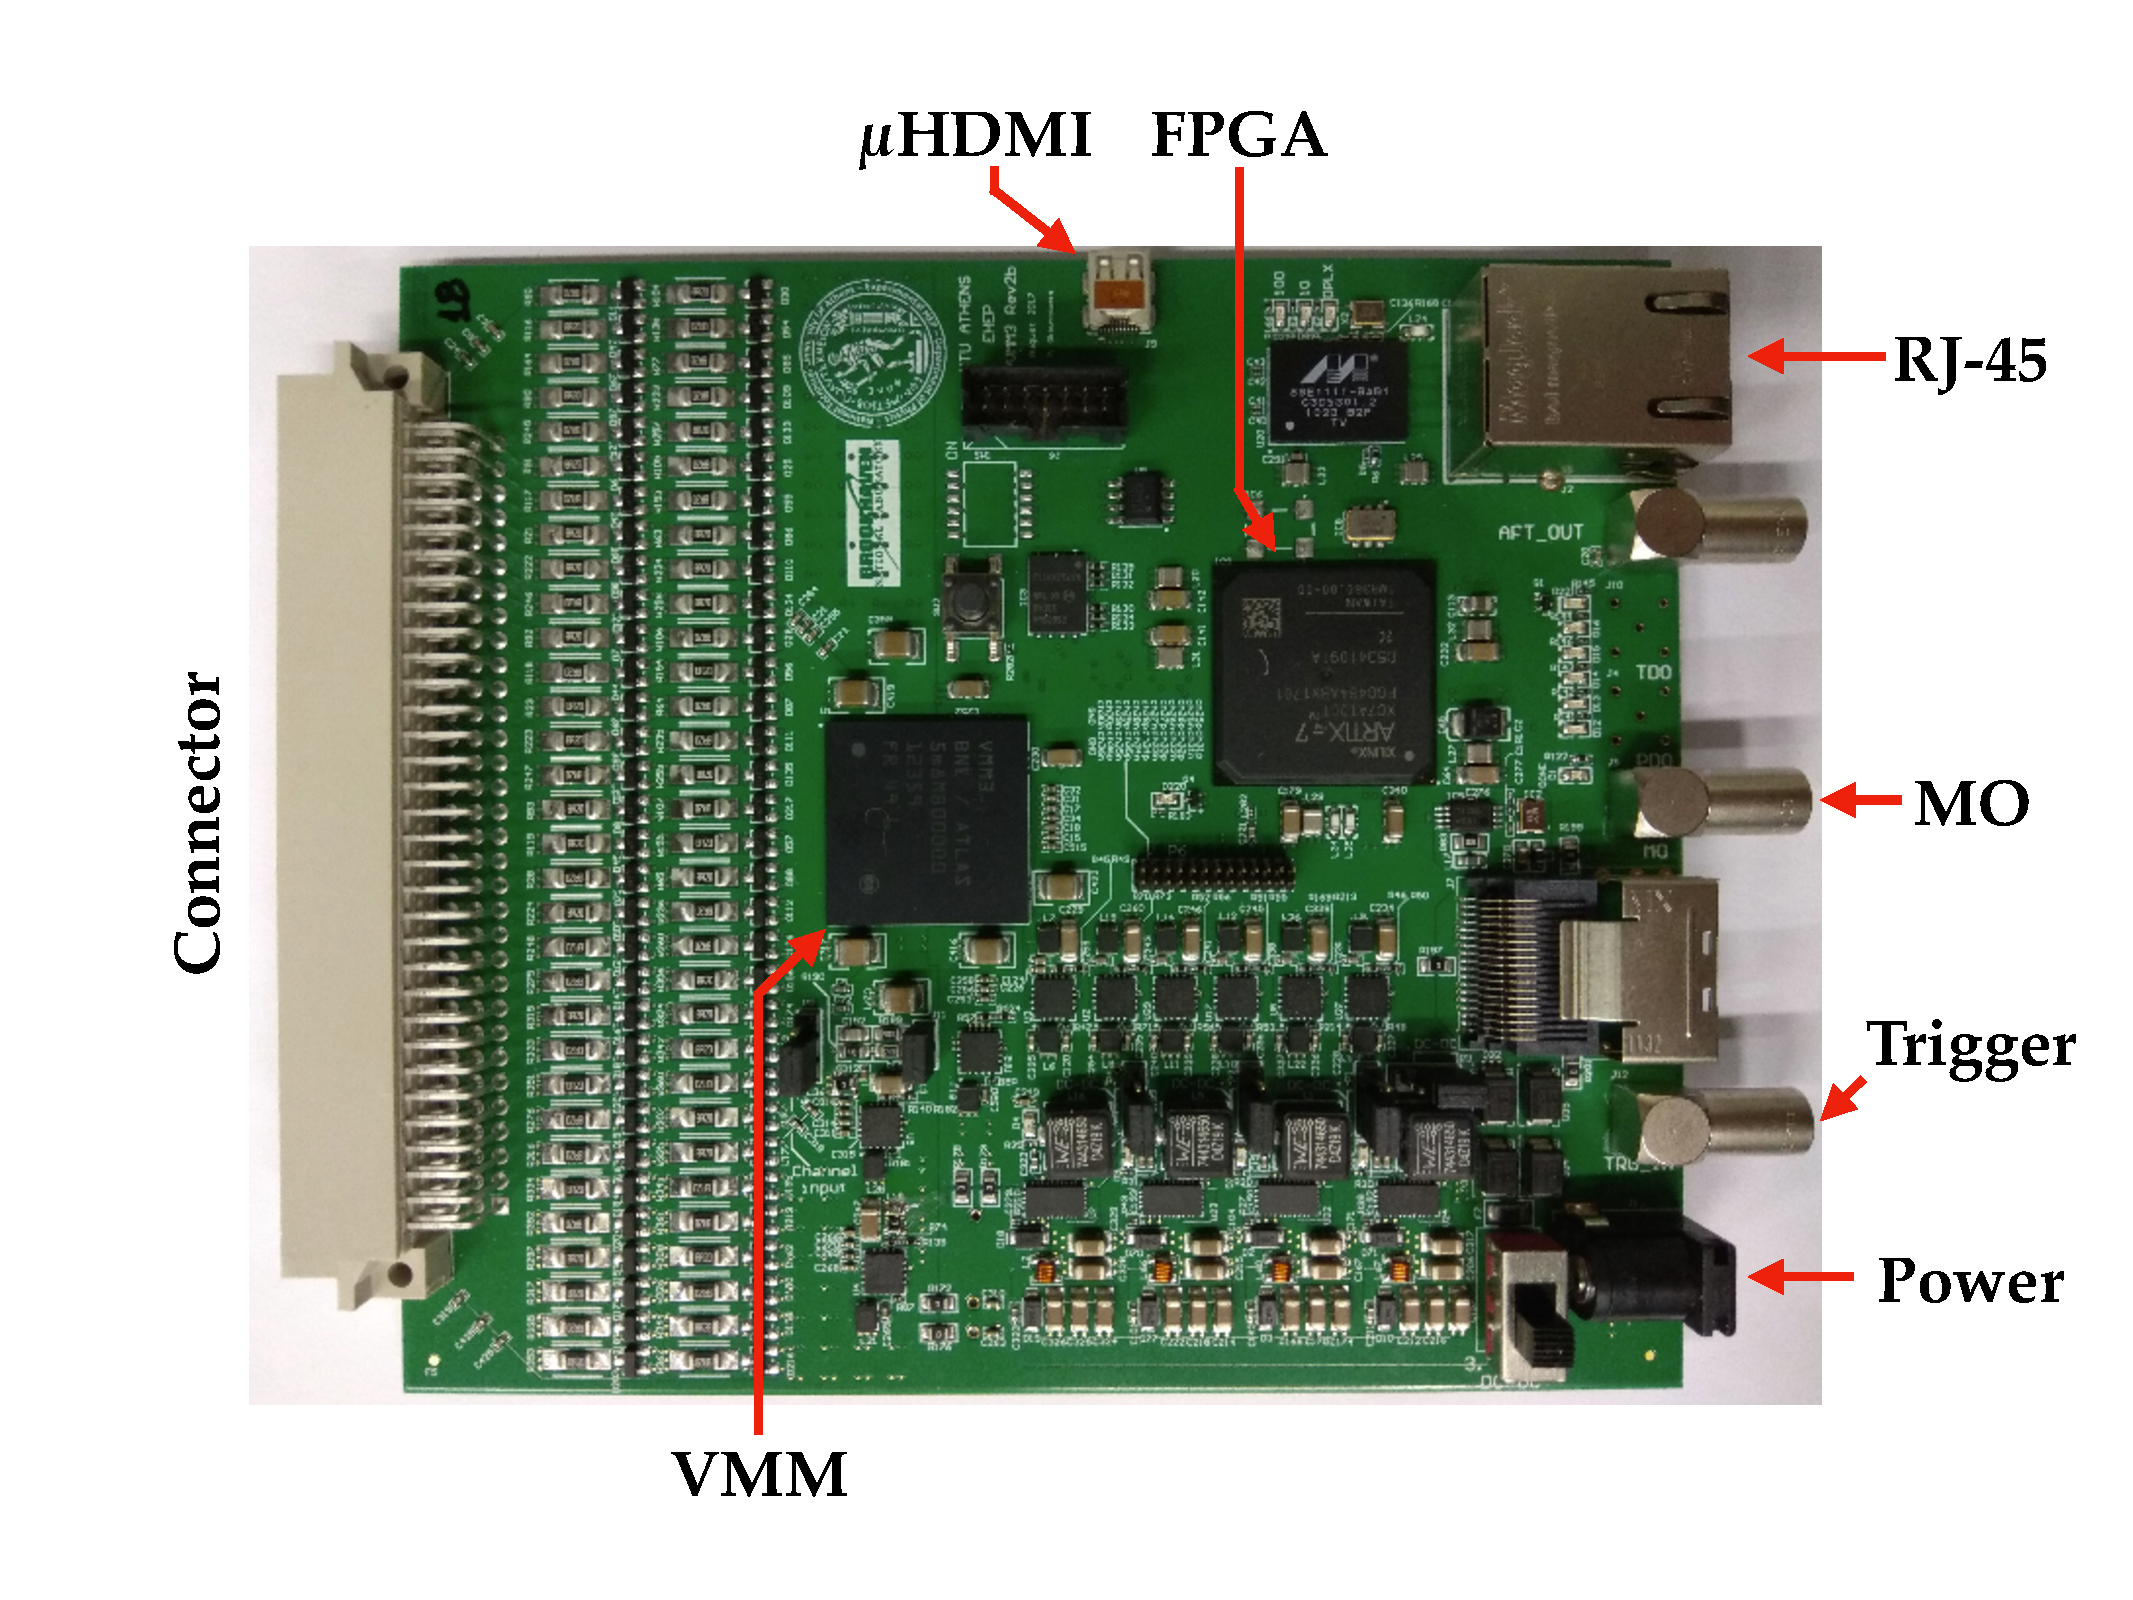
\includegraphics[width=0.8\textwidth]{figures/nsw/frontend/gpvmm_labelledPDF}
        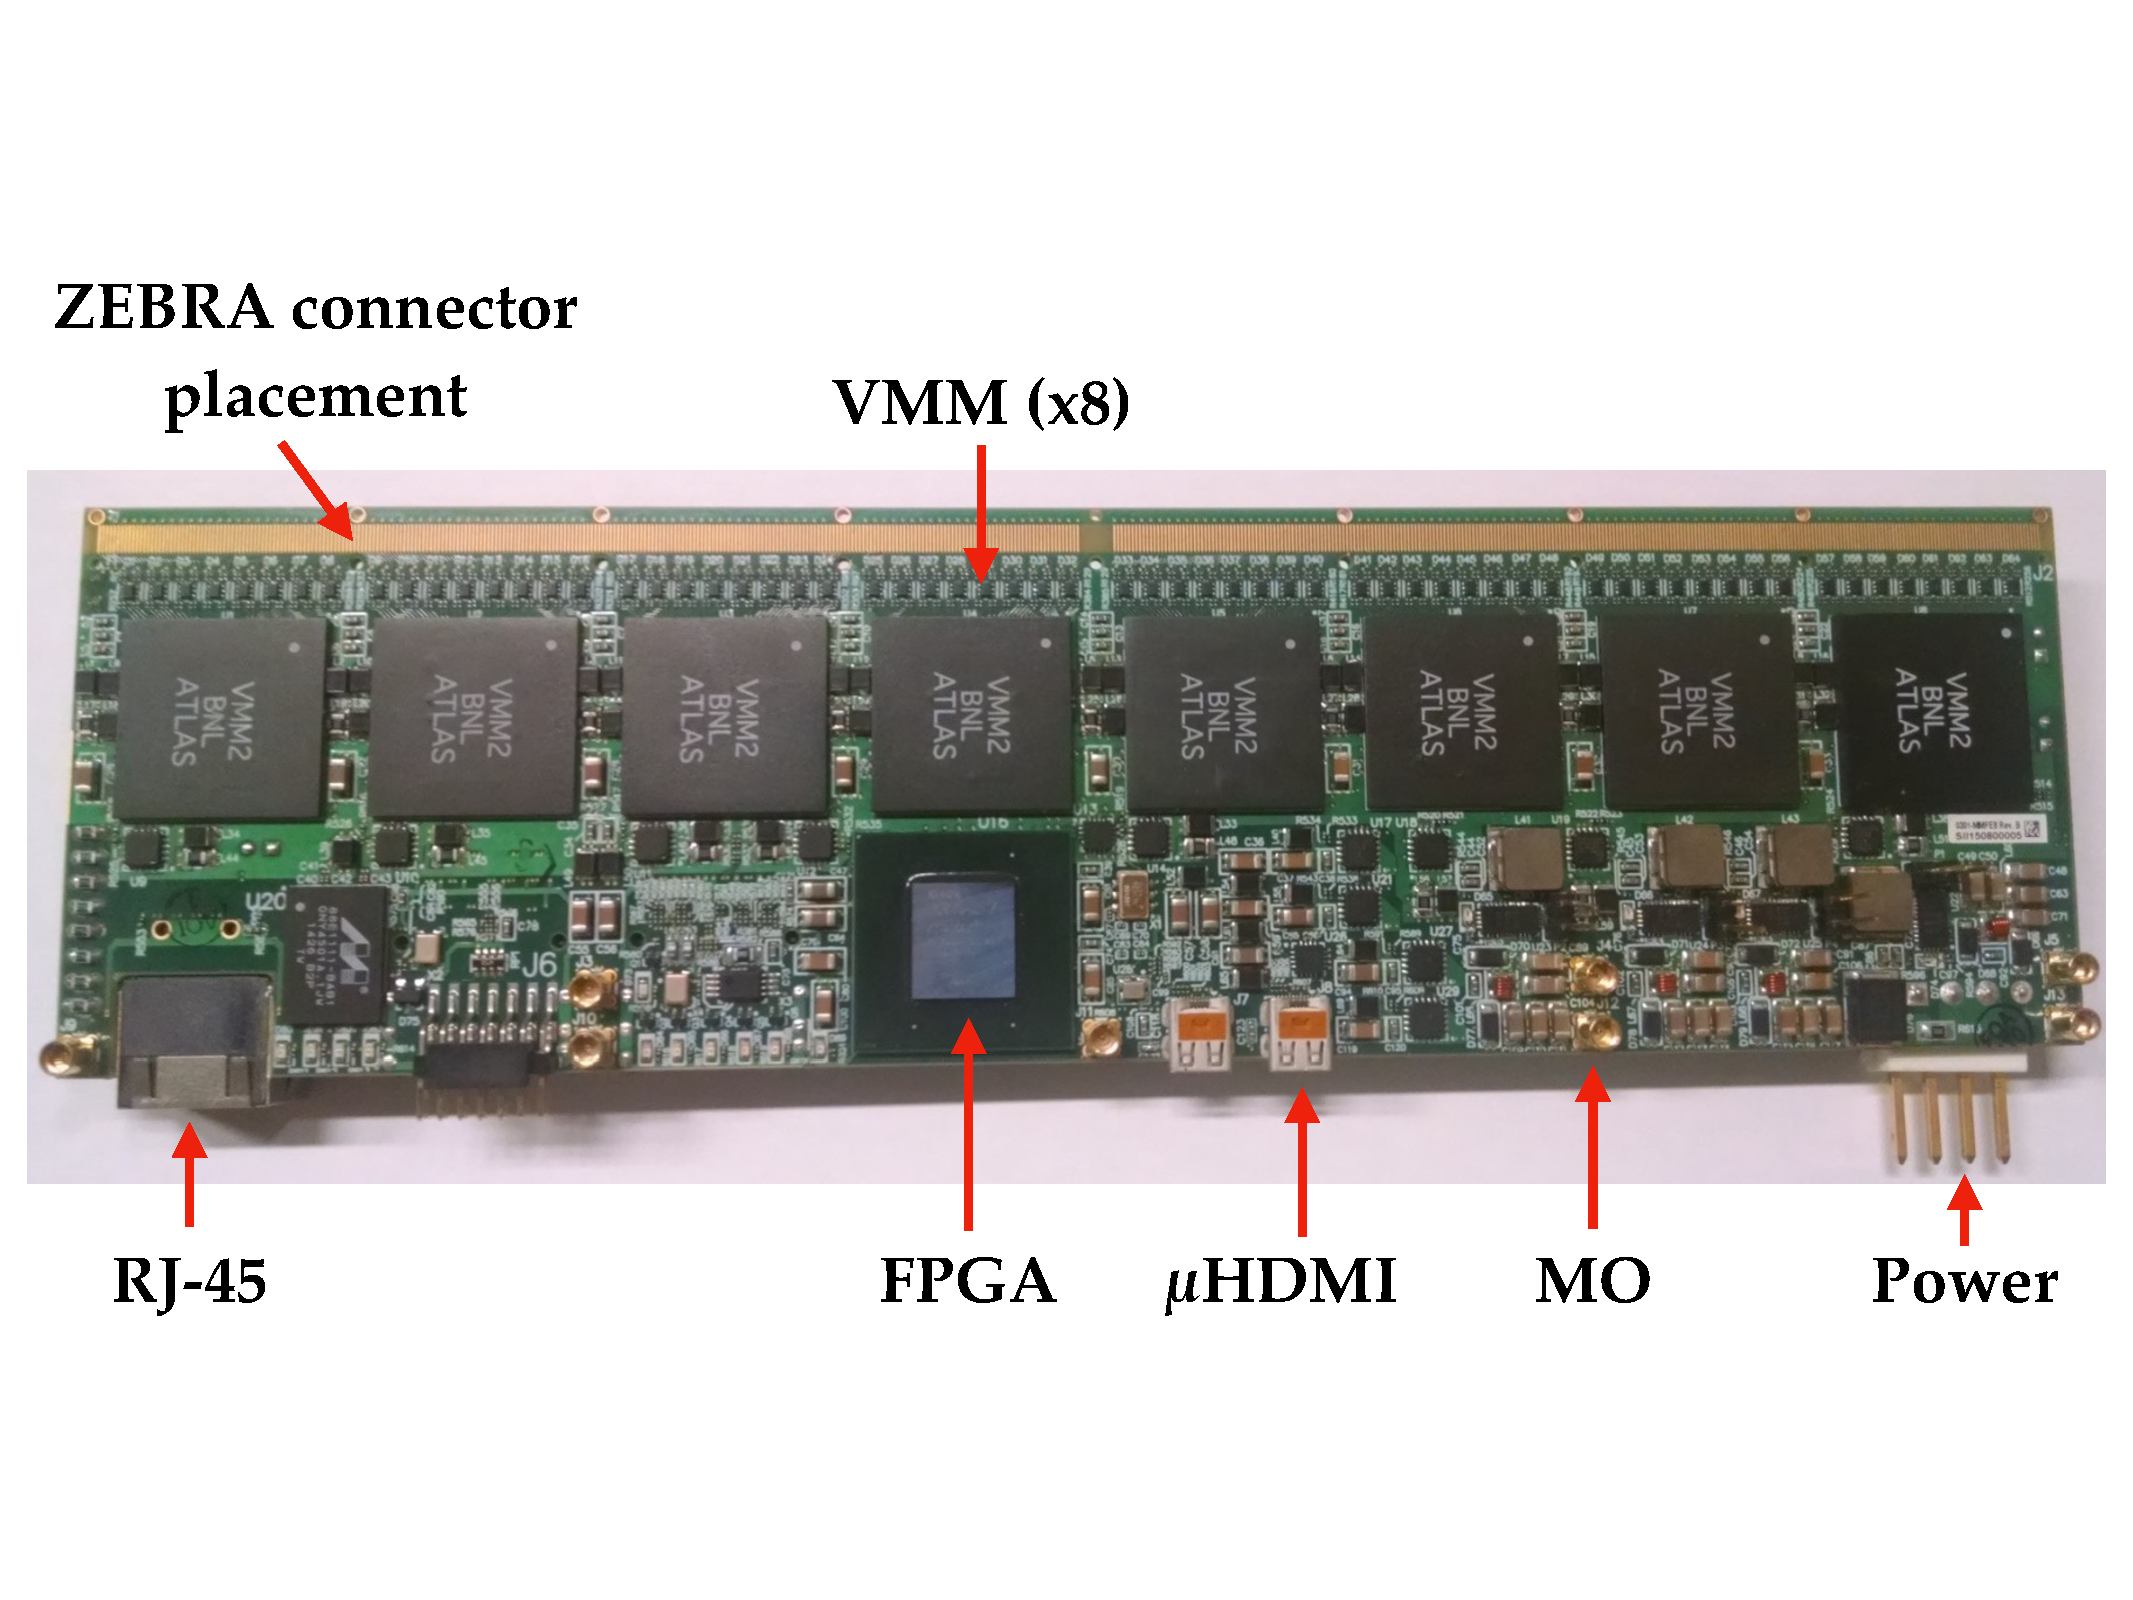
\includegraphics[width=0.8\textwidth]{figures/nsw/frontend/mmfe8_labelledPDF}
        \caption{
            Pictures of two VMM-based frontend boards. The RJ-45 connectors provide network I/O via
            standard Ethernet cables.
            The $\mu$HDMI connectors provide inputs for additional signalling purposes, such as external
            trigger signals.
            `MO' refers to the multiplexed monitoring output of the VMM (see Figure~\ref{fig:vmm3_channel}), which samples the analog
            signals internal to the VMM, such as the shaped input signals, prior to their digitisation.
            \textbf{\textit{Top}}: General purpose VMM (GPVMM) board housing a single VMM ASIC.
            The MO and trigger I/O are provided by LEMO connectors.
            \textbf{\textit{Bottom}}: Prototype MMFE8 board with its 8 VMM ASICs.
            The ZEBRA connector used for the MM detectors is described in the text.
            On this board the MO output is accessible primarily by the use of a oscilloscope probe.
        }
        \label{fig:frontend_boards}
    \end{center}
\end{figure}

\begin{figure}[!htb]
    \begin{center}
        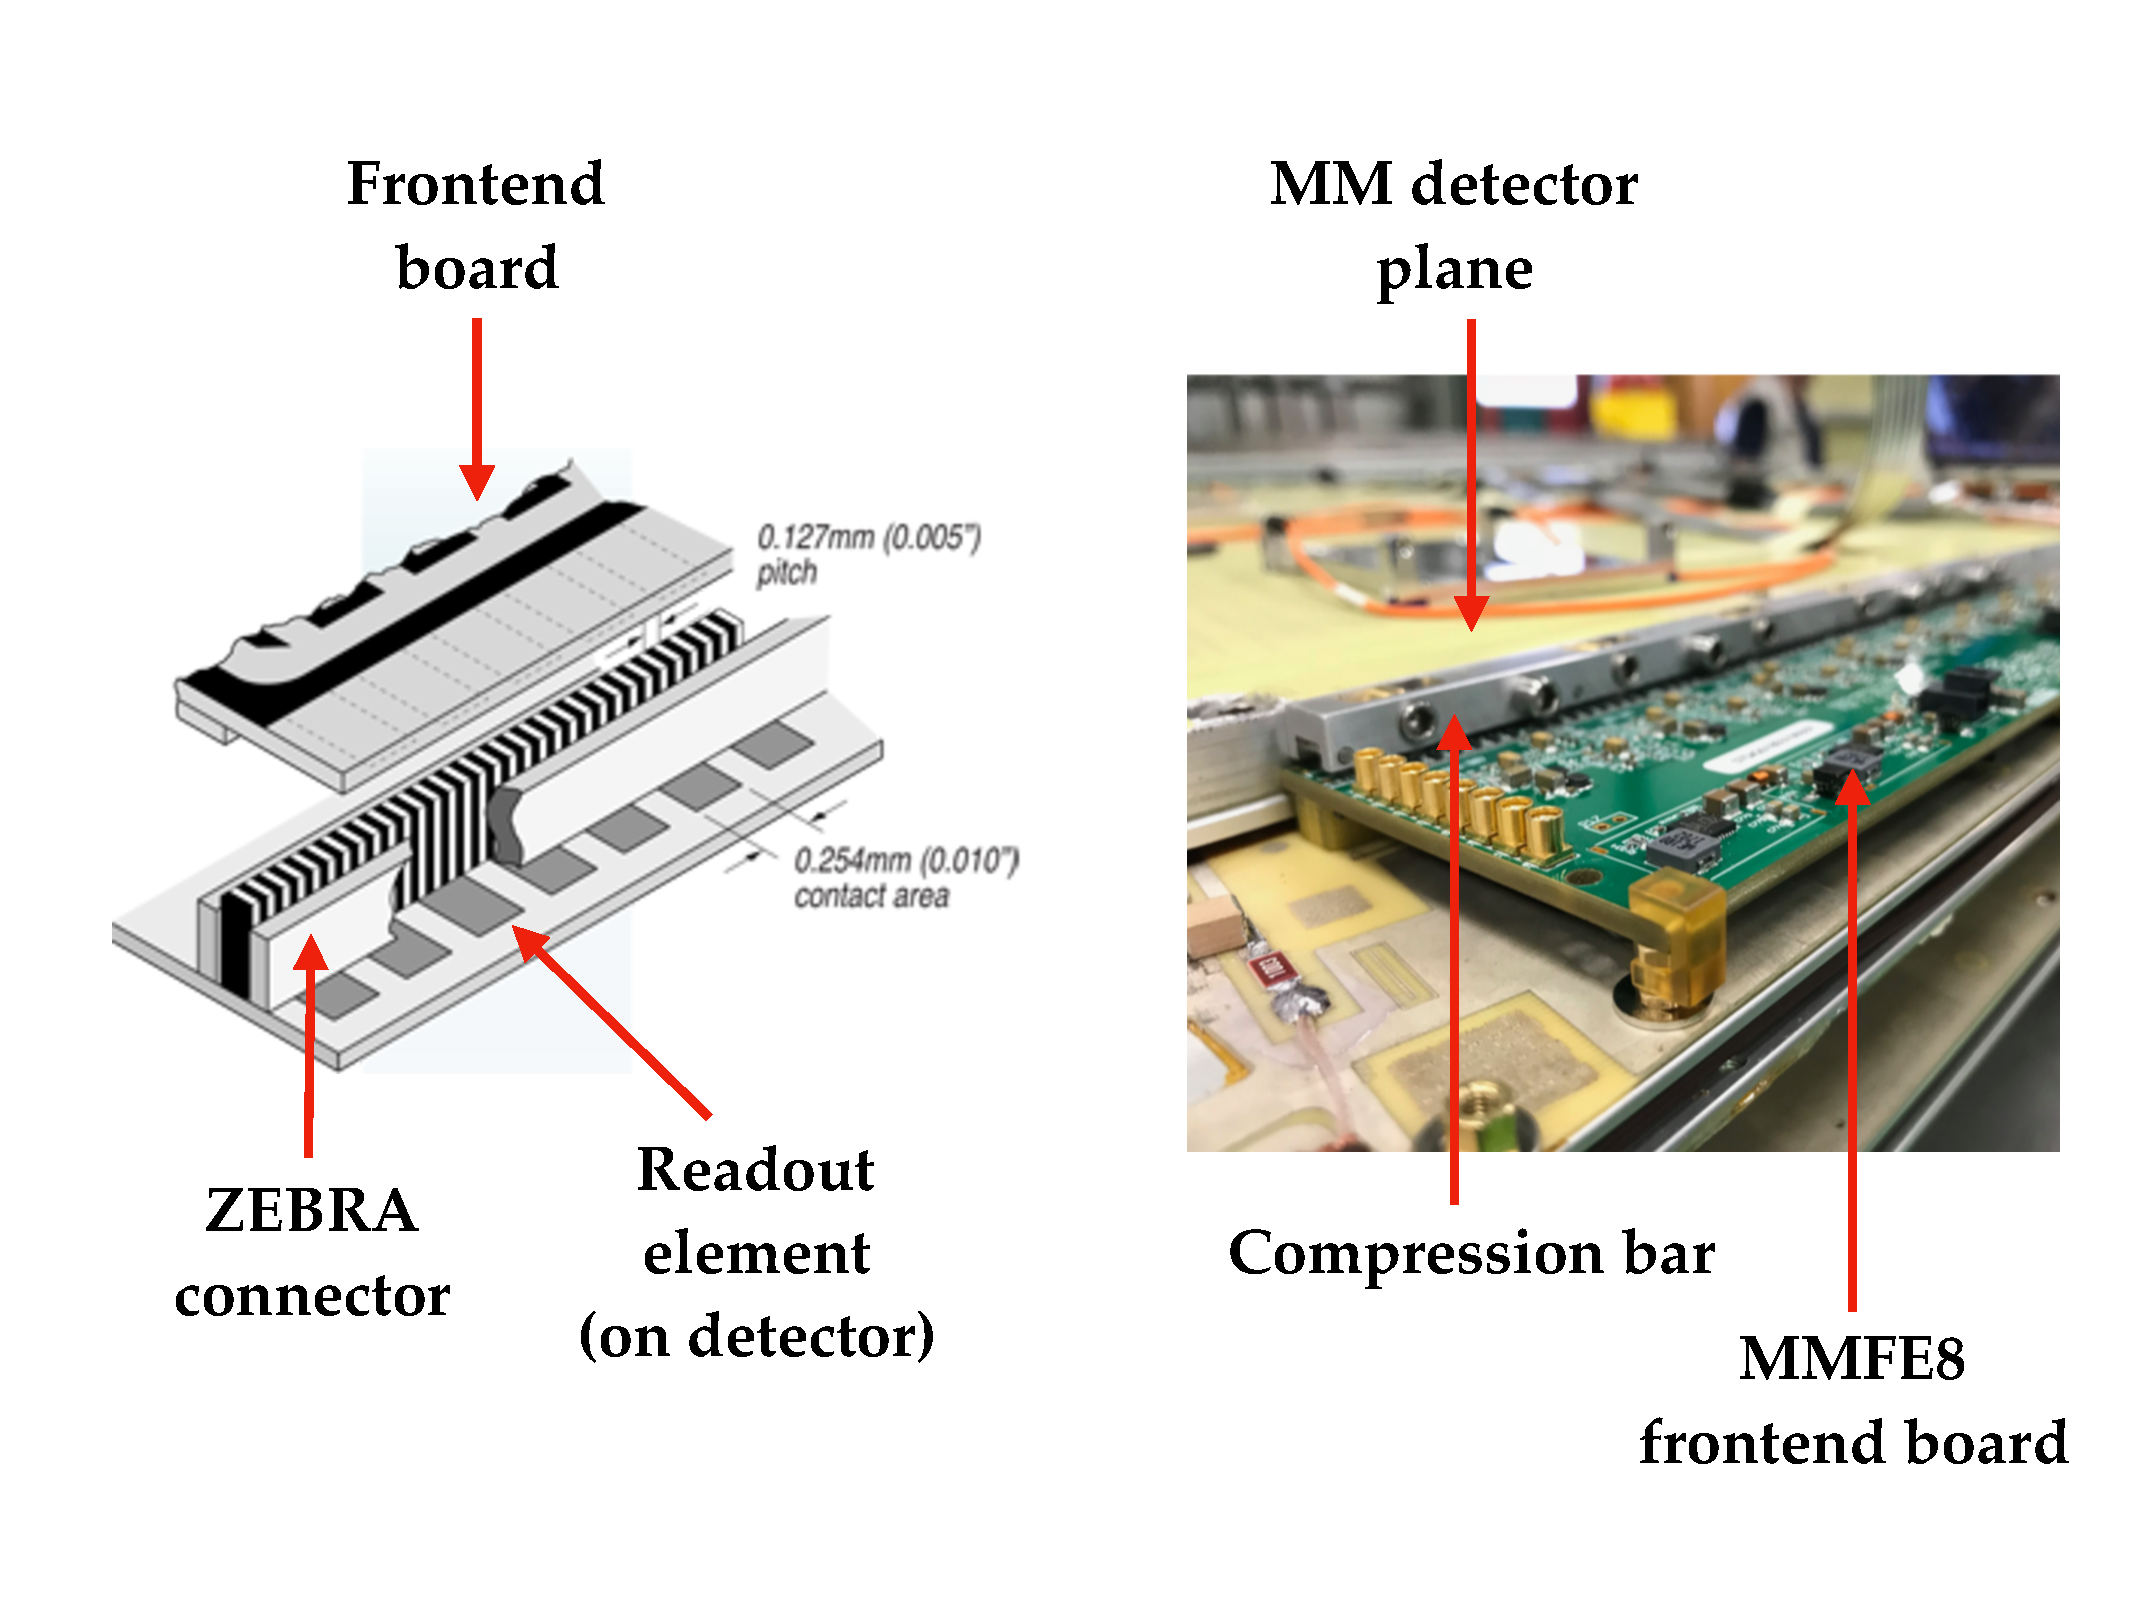
\includegraphics[width=0.8\textwidth]{figures/nsw/frontend/zebra_connector_illustratedPDF}
        \caption{
            \textbf{\textit{Left}}: Illustration of the ZEBRA connector concept.
                The ZEBRA connector is composed of a high density of alternating conductive (white) and non-conductive (black) layers
                that make contact with the detector readout elements on bottom and frontend board sensing elements
                on top.
            \textbf{\textit{Right}}: Picture of the ZEBRA connector being used with an MMFE8 frontend board
                on a full-scale MM detector.
                When interfaced to the MM detector, the MMFE8 frontend board is situated such that the VMMs are downward facing and
                are not therefore visible as pictured.
                The connection of the ZEBRA connector is realised via the tightening of a compression bar mounted on the MM detector chamber.
                The resulting
                downward pressure forces the ZEBRA connector to be securely sandwiched between
                the readout elements of the MM detector and VMM channel inputs located on the frontend board, bringing them in direct electrical contact.
        }
        \label{fig:zebra_connector}
    \end{center}
\end{figure}

The NSW frontend boards are interfaced directly to the detectors.
Both the GPVMM-type and MMFE8 frontend boards have been used on small prototype MM detectors, with
active area of $10\times10$\,cm$^2$.
A picture of an MMFE8 connected to such a detector is shown in Figure~\ref{fig:mmfe8_t2}.
On the full-scale MM detectors to be used in the NSW, the frontend boards are situated along the edge
of each detector layer in a given multilayer.
A drawing of a complete MM quadruplet with frontend electronics boards is shown in Figure~\ref{fig:mm_quad_elx}.


\begin{figure}[!htb]
    \begin{center}
        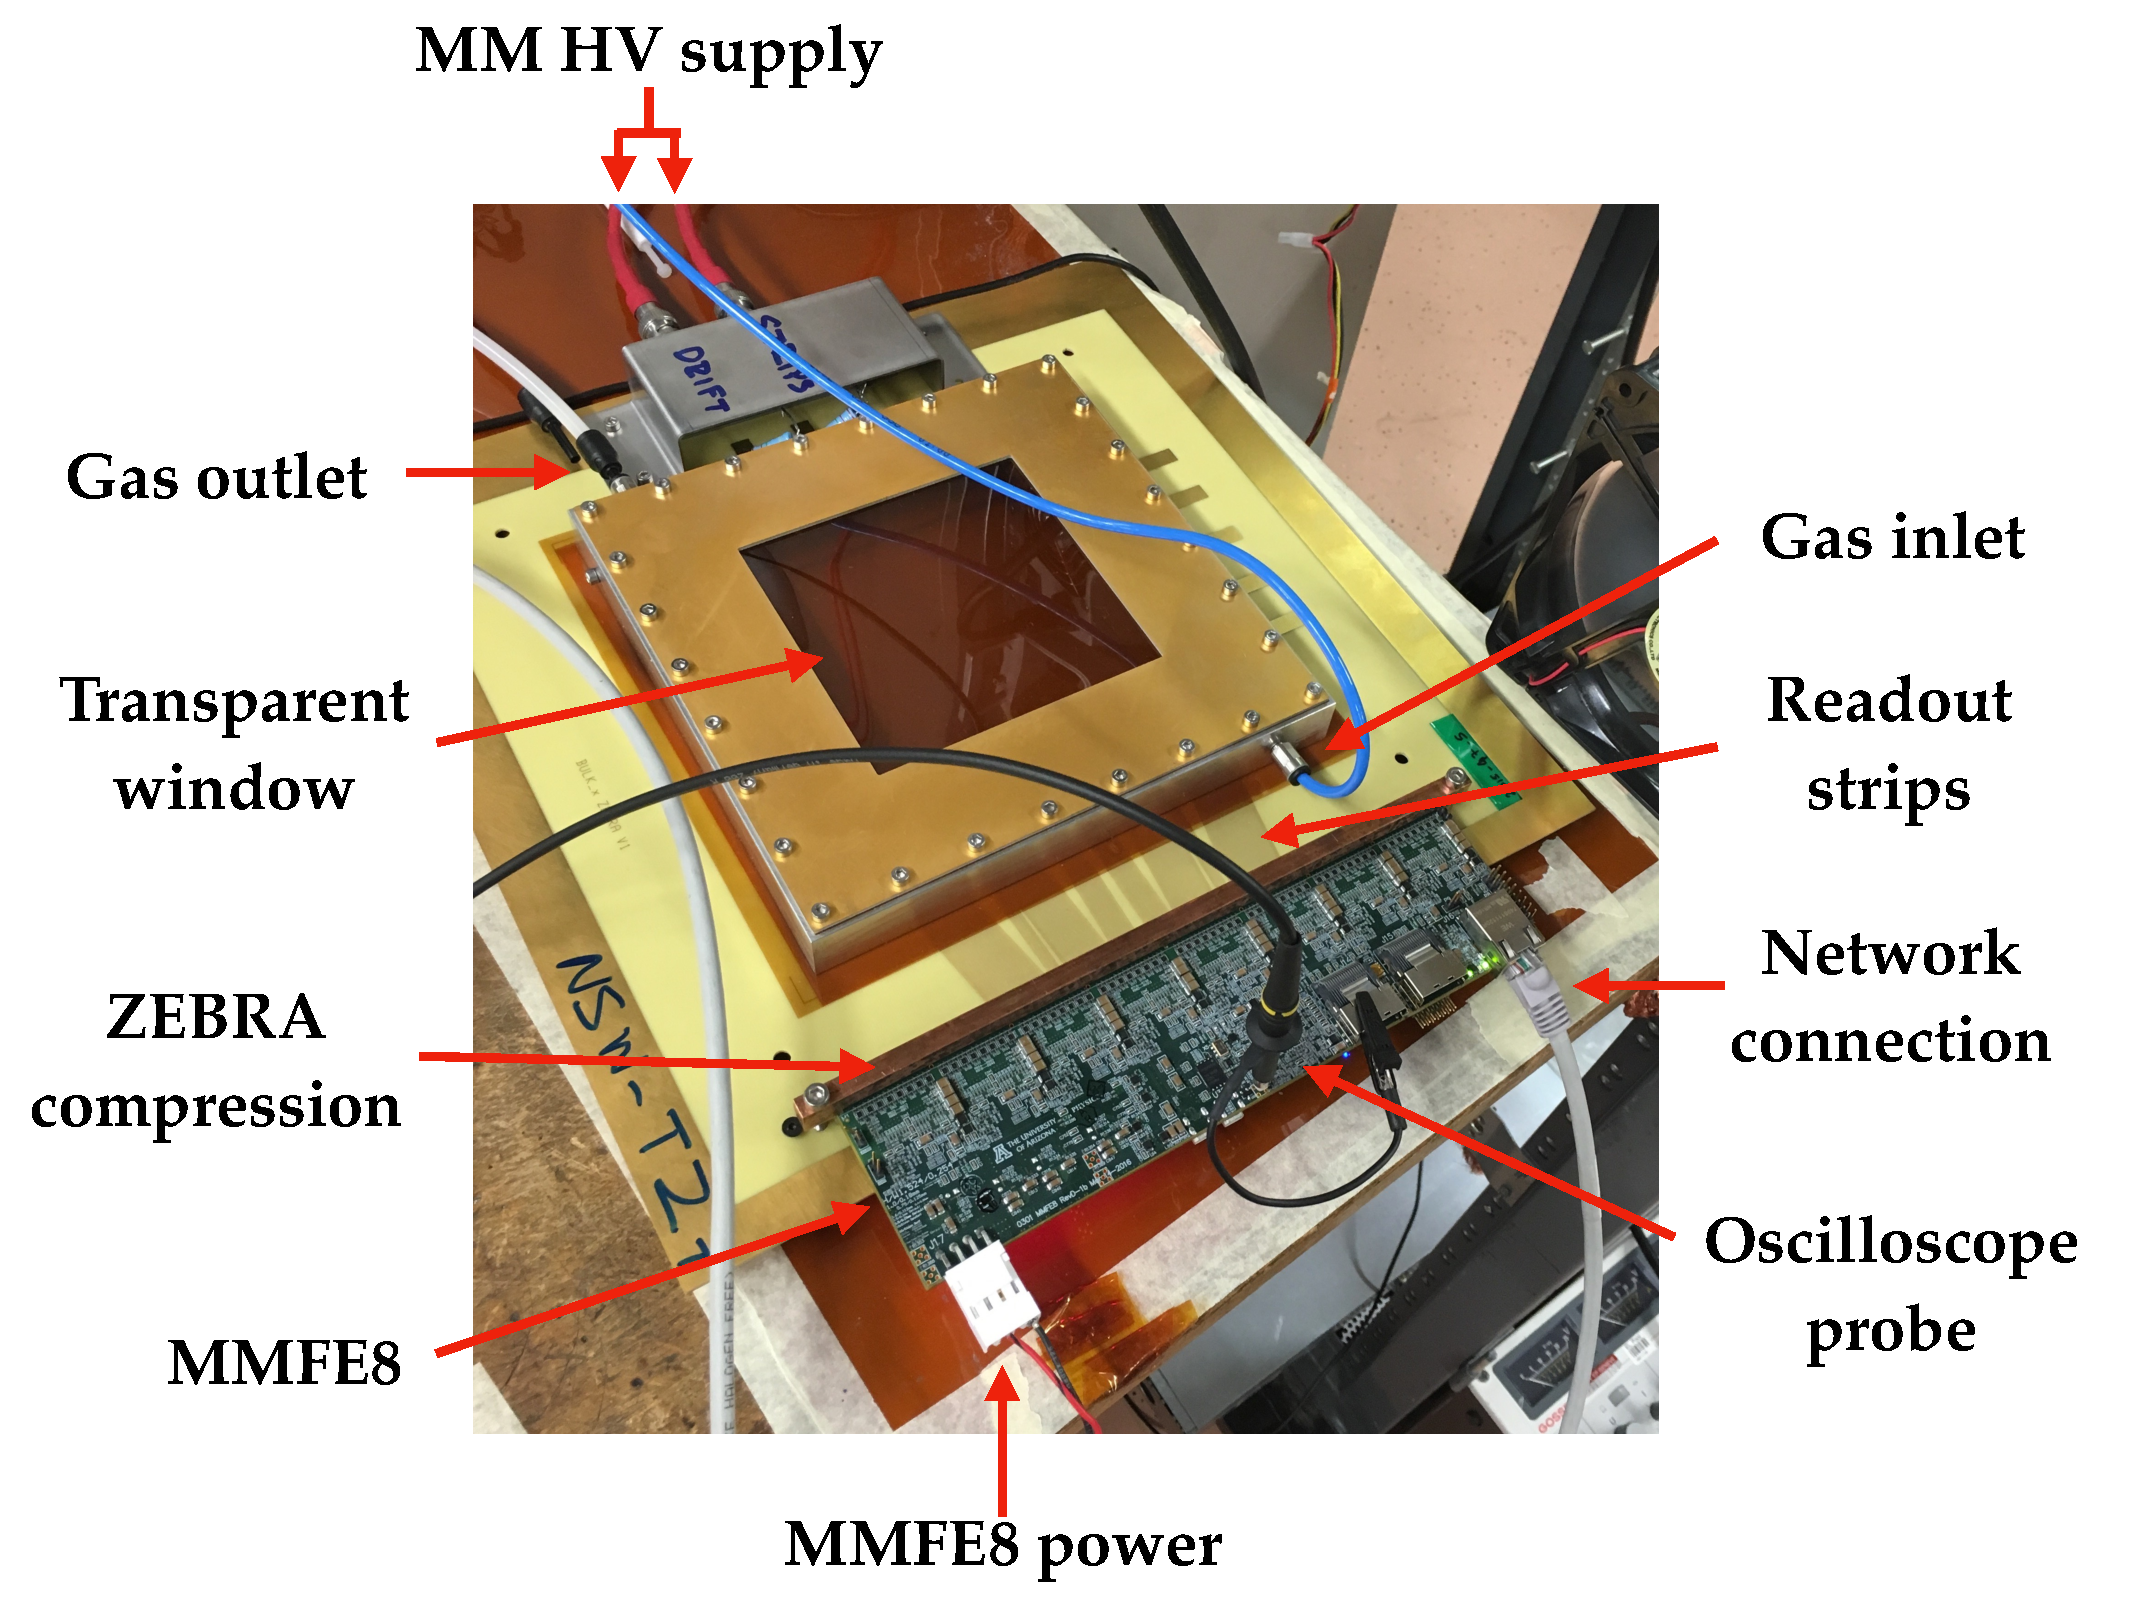
\includegraphics[width=0.75\textwidth]{figures/nsw/frontend/mmfe8_t2_labelledPDF}
        \caption{
        }
        \label{fig:mmfe8_t2}
    \end{center}
\end{figure}

\begin{figure}[!htb]
    \begin{center}
        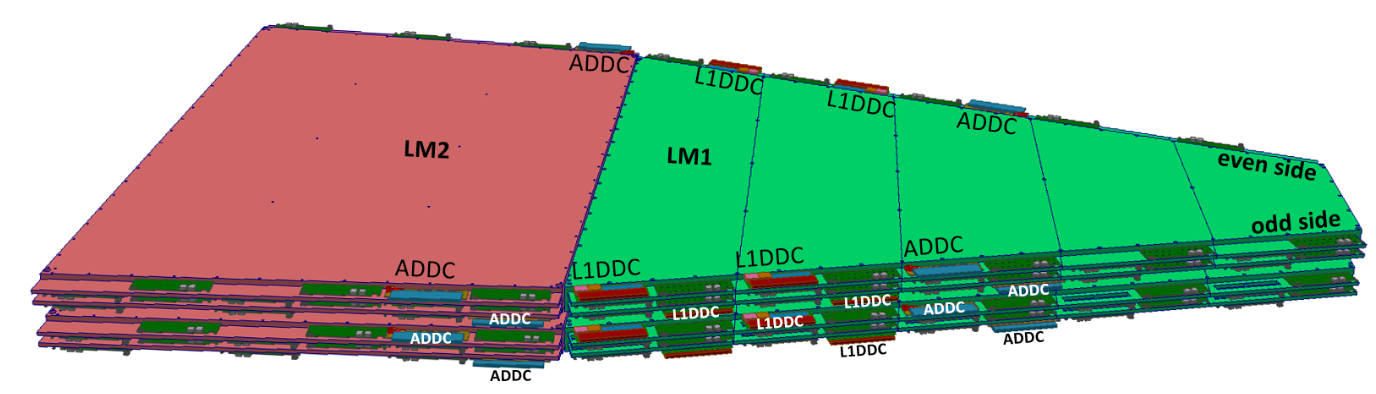
\includegraphics[width=0.8\textwidth]{figures/nsw/frontend/mm_quad_elx}
        \caption{
            {\color{red}{Explain how the frontend boards are situated on the NSW chambers}}
        }
        \label{fig:mm_quad_elx}
    \end{center}
\end{figure}

\FloatBarrier

\section{Configuration, Data-acquisition, and Calibration Software for the NSW Front-end Electronics}
\subsection{VERSO}
\subsection{Calibration Algorithm Development}
\subsubsection{Gain}
\subsubsection{ADC Calibration}
\subsubsection{Noise Measurements}
\subsubsection{Timing Calibration}
\subsubsection{Per-channel Threshold Equilisation}
\subsection{Use Cases}
\subsubsection{Test Benches and Labs}
\subsubsection{High Rate Tests and Test Beams}

\section{The Upgrade of the ATLAS T/DAQ Infrastructure}
\subsection{FELIX}
\subsection{The Software ROD}
